\documentclass{WileyMSP-template}

\usepackage{amsmath}
\usepackage{amssymb}


\begin{document}


\pagestyle{fancy}
\rhead{\includegraphics[width=2.5cm]{vch-logo.png}}


\title{Influence of illumination spectrum on dissociation kinetic of iron-boron pairs in silicon}

\maketitle



% Author: Please give full first and last names for authors and include * after the name of all corresponding authors

\author{Oleg Olikh*}
\author{Oleksandr Datsenko}
\author{Serhiy Kondratenko}

% Dedication

\dedication{}






% Affiliations: Please provide adacemic titles (Prof. or Dr.) for all authors where applicable, and include an institutional email address for all corresponding authors
\begin{affiliations}
Prof. O. Olikh, Dr. O. Datsenko, Prof. S. Kondratenko\\
Taras Shevchenko National University of Kyiv, 64/13, Volodymyrska Street, 01601, Kyiv, Ukraine\\
Email Address: olegolikh@knu.ua

%A. N. O. Author\\
%Address

\end{affiliations}


% Keywords: Please provide a minimum of three and a maximum of seven keywords, separated by commas

\keywords{silicon, iron-boron pairs, light-induced dissociation, wavelength impact, dissociation rate}



% Abstract should be written in the present tense and impersonal style (i.e., avoid we), and be at most 200 words long
\begin{abstract}

Herein, the results of an experimental study on the photo-dissociation kinetic of iron–boron (FeB) pairs
in boron-doped Czochralski silicon using different light sources are reported.
It was shown that the FeB dissociation rate depends not only on integrated light intensity
and overall carrier generation rate, but also on spectral composition of illumination.
The value of the material constant of dissociation $K$ varies and has been determined to be within $(1.5-3.8)\times10^{-15}$~s.
The investigation has revealed  increase in the dissociation rate with an increase in photon energy.
The results allowed us to conclude the dominant role of the recombination-enhanced defect reaction
at the second stage of the pair dissociation.

\end{abstract}


% Text: Please use section headings and subheadings as specified below. For communications, all section headings apart from Experimental Section should be removed
% Please make the first reference to a display item bold: \textbf{Figure 1}
% Do not abbreviate Figure, Equation, etc.; display items are always singular, i.e., Figure 1 and 2.
% Equations are always singular, i.e., Equation 1 and 2, and should be inserted using the {equation} environment, not as graphics
% Please do not use footnotes in the text, additional information can be added to the Reference list.


\section{Introduction}

Defects significantly impact semiconductor properties.
Although minimizing device dimensions to nanometers shifts some focus from extended to point defects,
physical properties still rely heavily on the presence and distribution of these irregularities.
Hence, many strategies for enhancing semiconductor structures, including radiation and temperature treatments or certain fabrication conditions, strive to decrease the defect concentration or neutralize its effects \cite{Cai2023,Vobecky2021,Frascaroli2021}.
For instance, in the case of photovoltaic devices, we must understand and optimize the carrier properties tied to defects and impurities  \cite{Cai2023}.
Such controlled alteration methods of the defective subsystem have been generalized under the term ``defect engineering'' and are extremely important from a practical standpoint.

Successful defect engineering hinges on an in-depth understanding of defect properties.
Key factors are defect formation energy, transition energy levels, self-compensating effects, nonradiative recombination caused by defects,
and the mechanism of reconstruction and diffusion  \cite{Cai2023}.
Considering the extraordinary diversity of possible intrinsic and impurity defects, complete information on all of them is lacking even for silicon, which is the most studied semiconductor.
Nevertheless, it must be noted that considerable data have been amassed on silicon, and have a solid understanding of some defects \cite{Juhl2018}.

For instance, such defects are iron impurity, a common, detrimental, and often unavoidable contaminant
in photovoltaic silicon \cite{Frascaroli2021,Sun2021}, and iron-boron pair.
Specifically, iron atoms are known to be at the interstitial sites, and Fe$_i^+$ are highly efficient recombination centers \cite{WeberFe}.
In p-type Si at room temperature, iron atoms are almost predominantly bound into complexes with dopants (B, Ga, Al, In).
This defect demonstrates bistable behavior: the stable state is defined by the configuration in which the Fe occupies
the first nearest tetrahedral interstitial site closest to the substituent atom,
whereas, in the metastable configuration, Fe is at the second $T_d$ interstitial site \cite{FeB:PhysRevB49}.
The energy levels associated with iron and its complexes, as well as the respective carriers capture cross-sections, are well-established \cite{Juhl2018,ROUGIEUX2018}.
Among the acceptor-iron pairs, the complex FeB is the most thoroughly investigated,
primarily due to the widespread use of Si:B in the fabrication of various devices, such as solar cells.
However, it is worth mentioning that gallium is gaining increasing attention as an acceptor dopant whose incorporation,
for instance, can help to mitigate the light and elevated temperature-induced degradation \cite{Ning2022}.

The dynamics of FeB pairs are also examined.
It's established that FeB pairs can be dissociated through illumination, minority carrier injection, and thermal treatment at 200~$^\circ$C \cite{FeBAssJAP2014}.
In the context of illumination, the dissociation rate $R_d$ is influenced by the overall carrier generation rate $G$ \cite{FeBLight2,FeBAssJAP2014,FeBKin2019,FeMethod2012}:
\begin{equation}
\label{eqRd}
R_d=K\left(\frac{G}{N_\mathrm{FeB}}\right)^2\,,
\end{equation}
where
$N_\mathrm{FeB}$ is the pair concentration,
$K$ is the constant of material.
To achieve almost complete dissociation of the FeB pairs, it is necessary for the illumination power to exceed 0.1~W~cm$^{-2}$ \cite{Macdonald2004}.
The dissociation process of FeB pairs by electron capture unfolds in two stages \cite{KIMERLINGFeB,FeBAssJAP2014}:
the initial stage involves the neutralization of Fe and the elimination of the Coulombic attraction between the pair components.
The mechanism of the second stage is contentious; it may involve either the recharge of the iron ion or the recombination-enhanced defect reaction
(REDR) triggered by electron-hole recombination.


It should be noted that despite the extensive data on the properties of iron-related defects in silicon, intensive research persists.
In particular, efforts focus on analyzing the impact of high-intensive  illumination \cite{FeBStrongIll}
or dopant compensation \cite{Zhu2015},
alongside clarifying the second-stage mechanism of dissociation \cite{Sun2021}
or reassessing recombination parameters \cite{Le2024}.

This study aims to investigate the effect of the light spectrum on the dissociation kinetics of FeB pairs in silicon.
While pair dissociation is typically carried out using a halogen lamp \cite{FeBLight2,Sun2021}
or 904 nm laser \cite{FeBStrongIll,FeBAssJAP2014,lauer2016}, there is limited understanding of how the light source influences this process.
By studying the impact of different illumination spectra on FeB dissociation,
we aim to provide valuable insights for defect engineering and the efficient transformation of detrimental impurity iron atoms into a highly mobile interstitial state
within the active region of a silicon device.
Besides, such information, in our opinion, can help make the right choice between existing options for the second stage of pair decay.

In \textbf{Figure~\ref{fig1}}, the main stages of the research are illustrated.
First step was determination of the dissociation rate of FeB pairs under illumination with different integral intensities.
Three light sources from different manufacturers were used (further details are described in Section~\ref{SecExp}).
To measure number of interstitial iron atoms formed over fixed time under strong illumination the kinetics of short-circuit current was used.
The result is presented in Subsection~\ref{SecR}.
Subsection~\ref{SecG} deals with estimating the carrier generation rate using spectra of sample illumination and considering the effects of light reflection,
absorption by free carriers, and effective absorption depths.
The obtained results showed that the efficiency of light-induced dissociation increases with decreasing photon wavelength --- see Subsection~\ref{SecLast}.
Finally, we conclude this paper in Section~\ref{SecConsl}.

\begin{figure}
\centering
  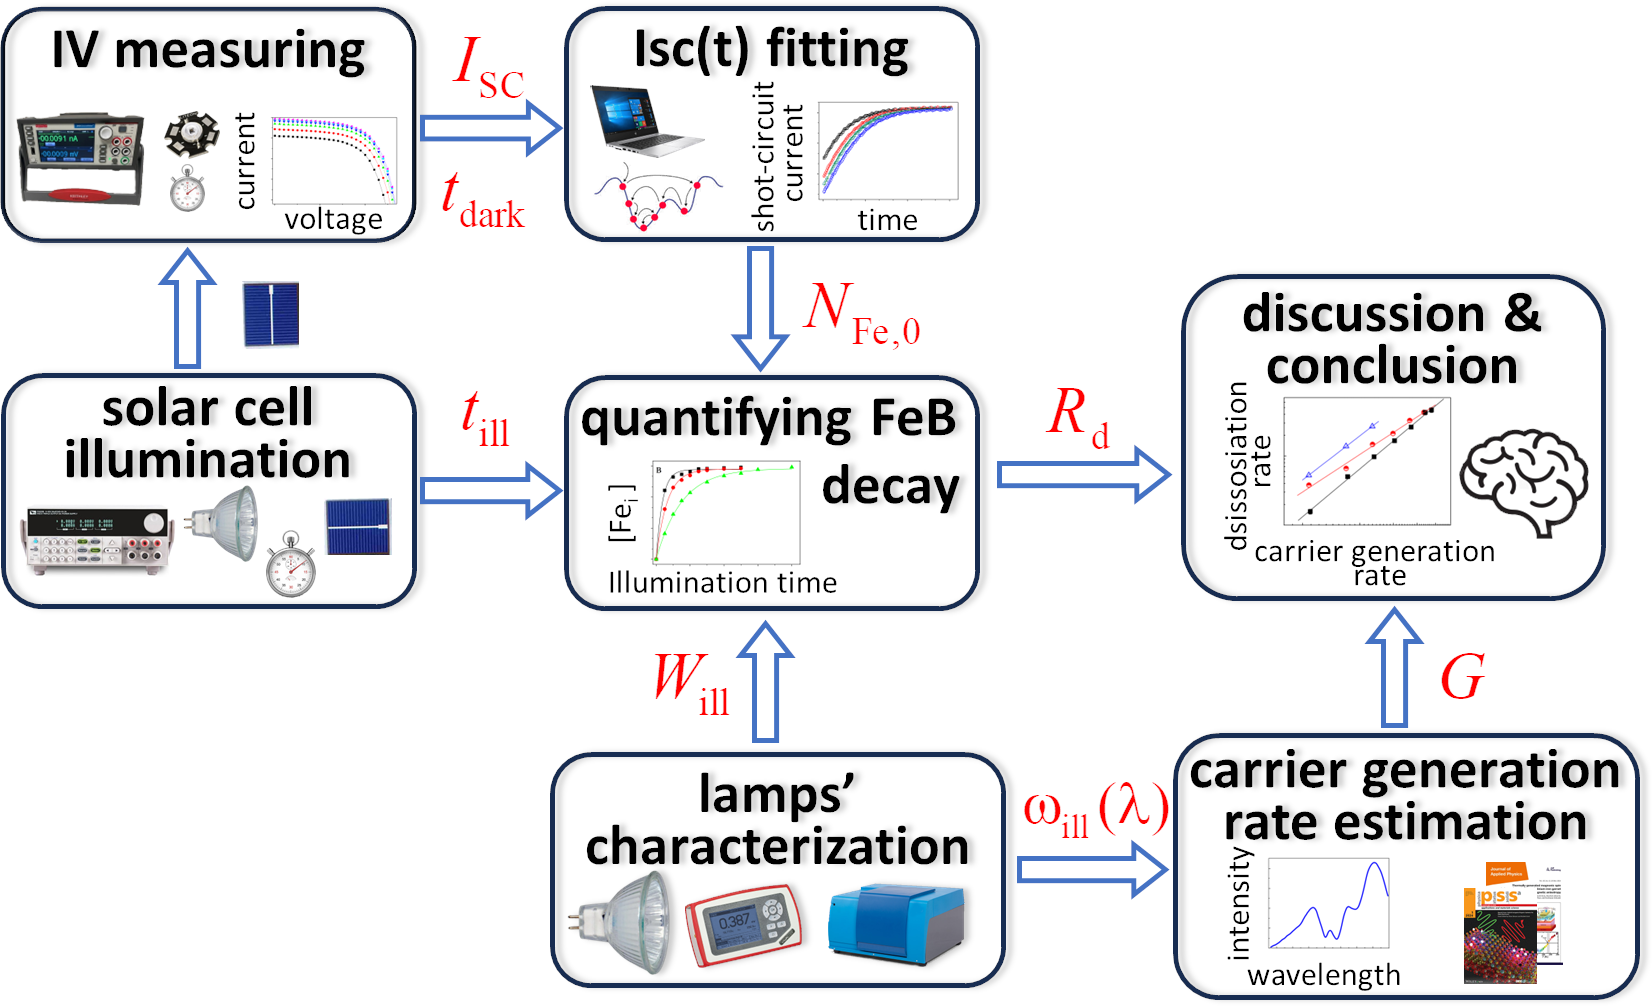
\includegraphics[width=0.5\linewidth]{Fig1.png}
  \caption{Investigation framework}
  \label{fig1}
\end{figure}



%\subsection{First Subsection}
%
%
%\subsubsection{First Sub Subsection}
%
%
%\threesubsection{First lowest-level subsection}


\section{Results and Discussion}

\subsection{Dissociation rate determination}\label{SecR}

The equilibrium between free Fe$_i$ and Fe$_i$B$_\mathrm{Si}$ is known to be determined by the following equations \cite{FeB:kinetic,Sun2021,FeBAssJAP2014}
\begin{equation}
\label{eqReac}
\mathrm{Fe}_i+\mathrm{B}_\mathrm{Si}  \overset{R_a}{\underset{R_d}{\rightleftharpoons{}}} \mathrm{FeB}\,,
\end{equation}
where
$R_a$ is the association rate.
As a result, the concentration of unpaired interstitial iron atoms $N_\mathrm{Fe_i}$ depending on illumination time $t_\mathrm{ill}$
during light-induced dissociation can be described as follows \cite{FeBLight2,FeBKin2019,Olikh2021JAP}
\begin{equation}
\label{eqNfeill}
N_\mathrm{Fe_i}(t_\mathrm{ill})=\left(N_\mathrm{Fe,eq}-N_\mathrm{Fe,tot}
\frac{R_d}{R_d+R_a}\right)\exp[-(R_d+R_a)t_\mathrm{ill}]+N_\mathrm{Fe,tot}\frac{R_d}{R_d+R_a}\,,
\end{equation}
where
$N_\mathrm{Fe,tot}$ is the total concentration of the impurity iron,
$N_\mathrm{Fe,eq}$ represents the concentration of unpaired interstitial iron atoms in the equilibrium state
(in darkness, $N_\mathrm{Fe,eq}=N_\mathrm{Fe_i}(t_\mathrm{ill}\leq0)$).
It's important to highlight that $N_\mathrm{Fe,eq}$ is significantly influenced
by temperature and the Fermi level location \cite{FeB:kinetic}.
Specifically, in the case of p-type Si with a hole concentration of $1.36\times10^{15}$~cm$^{-3}$
(which corresponds to the base of the structure under investigation),
at a temperature of $T=300$~K, $N_\mathrm{Fe,eq}$ constitutes merely about 1\% of $N_\mathrm{Fe,tot}$,
rendering it negligible for practical considerations.
However, when the temperature rises to 340~K, the proportion of $N_\mathrm{Fe,eq}$ increases to approximately 14.5\%.

After the cessation of illumination, only the process of association occurs,
and the time dependence of Fe$_i$ concentration can be expressed as follows \cite{FeB:kinetic,MurphyJAP2011}:
\begin{equation}
\label{eqNFet}
N_\mathrm{Fe_i}(t_\mathrm{dark})=(N_\mathrm{Fe,0}-N_\mathrm{Fe,eq})\times
\exp(-R_a t_\mathrm{dark})+N_\mathrm{Fe,eq}\,,
\end{equation}
where $t_\mathrm{dark}$ is the time after stopping of strong illumination,
$N_\mathrm{Fe,0}$ is the concentration of interstitial iron atoms formed after illumination,
$N_\mathrm{Fe,0}=N_\mathrm{Fe_i}(t_\mathrm{dark}=0)=N_\mathrm{Fe_i}(t_\mathrm{ill})$.

The study examined the dependence of $N_\mathrm{Fe,0}$ in silicon solar cells on illumination time $t_\mathrm{ill}$
using different integral illumination intensities $W_\mathrm{ill}$ ($200-750$~mW) and light sources
(three halogen lamps, labeled as Orion, Osram, and GE, and described in detail in Section~\ref{SecExp}).
The experiments were conducted at a temperature of 340~K.
The values of $N_\mathrm{Fe,0}$ were  determined using a methodology \cite{Olikh2022:JMatSci,Olikh2021JAP}
based on the fitting of the kinetics of short-circuit current $I_{SC}$ under low-intensity monochromatic illumination.
Specifically, after strong illumination with a duration of $t_\mathrm{ill}$,
the current-voltage characteristic ($I$-$V$) of the solar cell was measured every 21 seconds over a time $t_\mathrm{dark}$ interval of approximately 3000 seconds.

\textbf{Figure~\ref{fig2}a} shows some typical $I$-$V$ curves.
It can be seen that upon cessation of illumination, there exists a gradual augmentation in both the short-circuit current and the open-circuit voltage.
This phenomenon is indicative of a decrease in the recombination activity of the defective subsystem,
which is a result of the transition of interstitial iron to a bound state with an acceptor.
Moreover, at the end of the measurement interval, the minute changes in the $I$-$V$ curves denote that the selected interval of 50 minutes is sufficient to complete the association.


\begin{figure}
\centering
  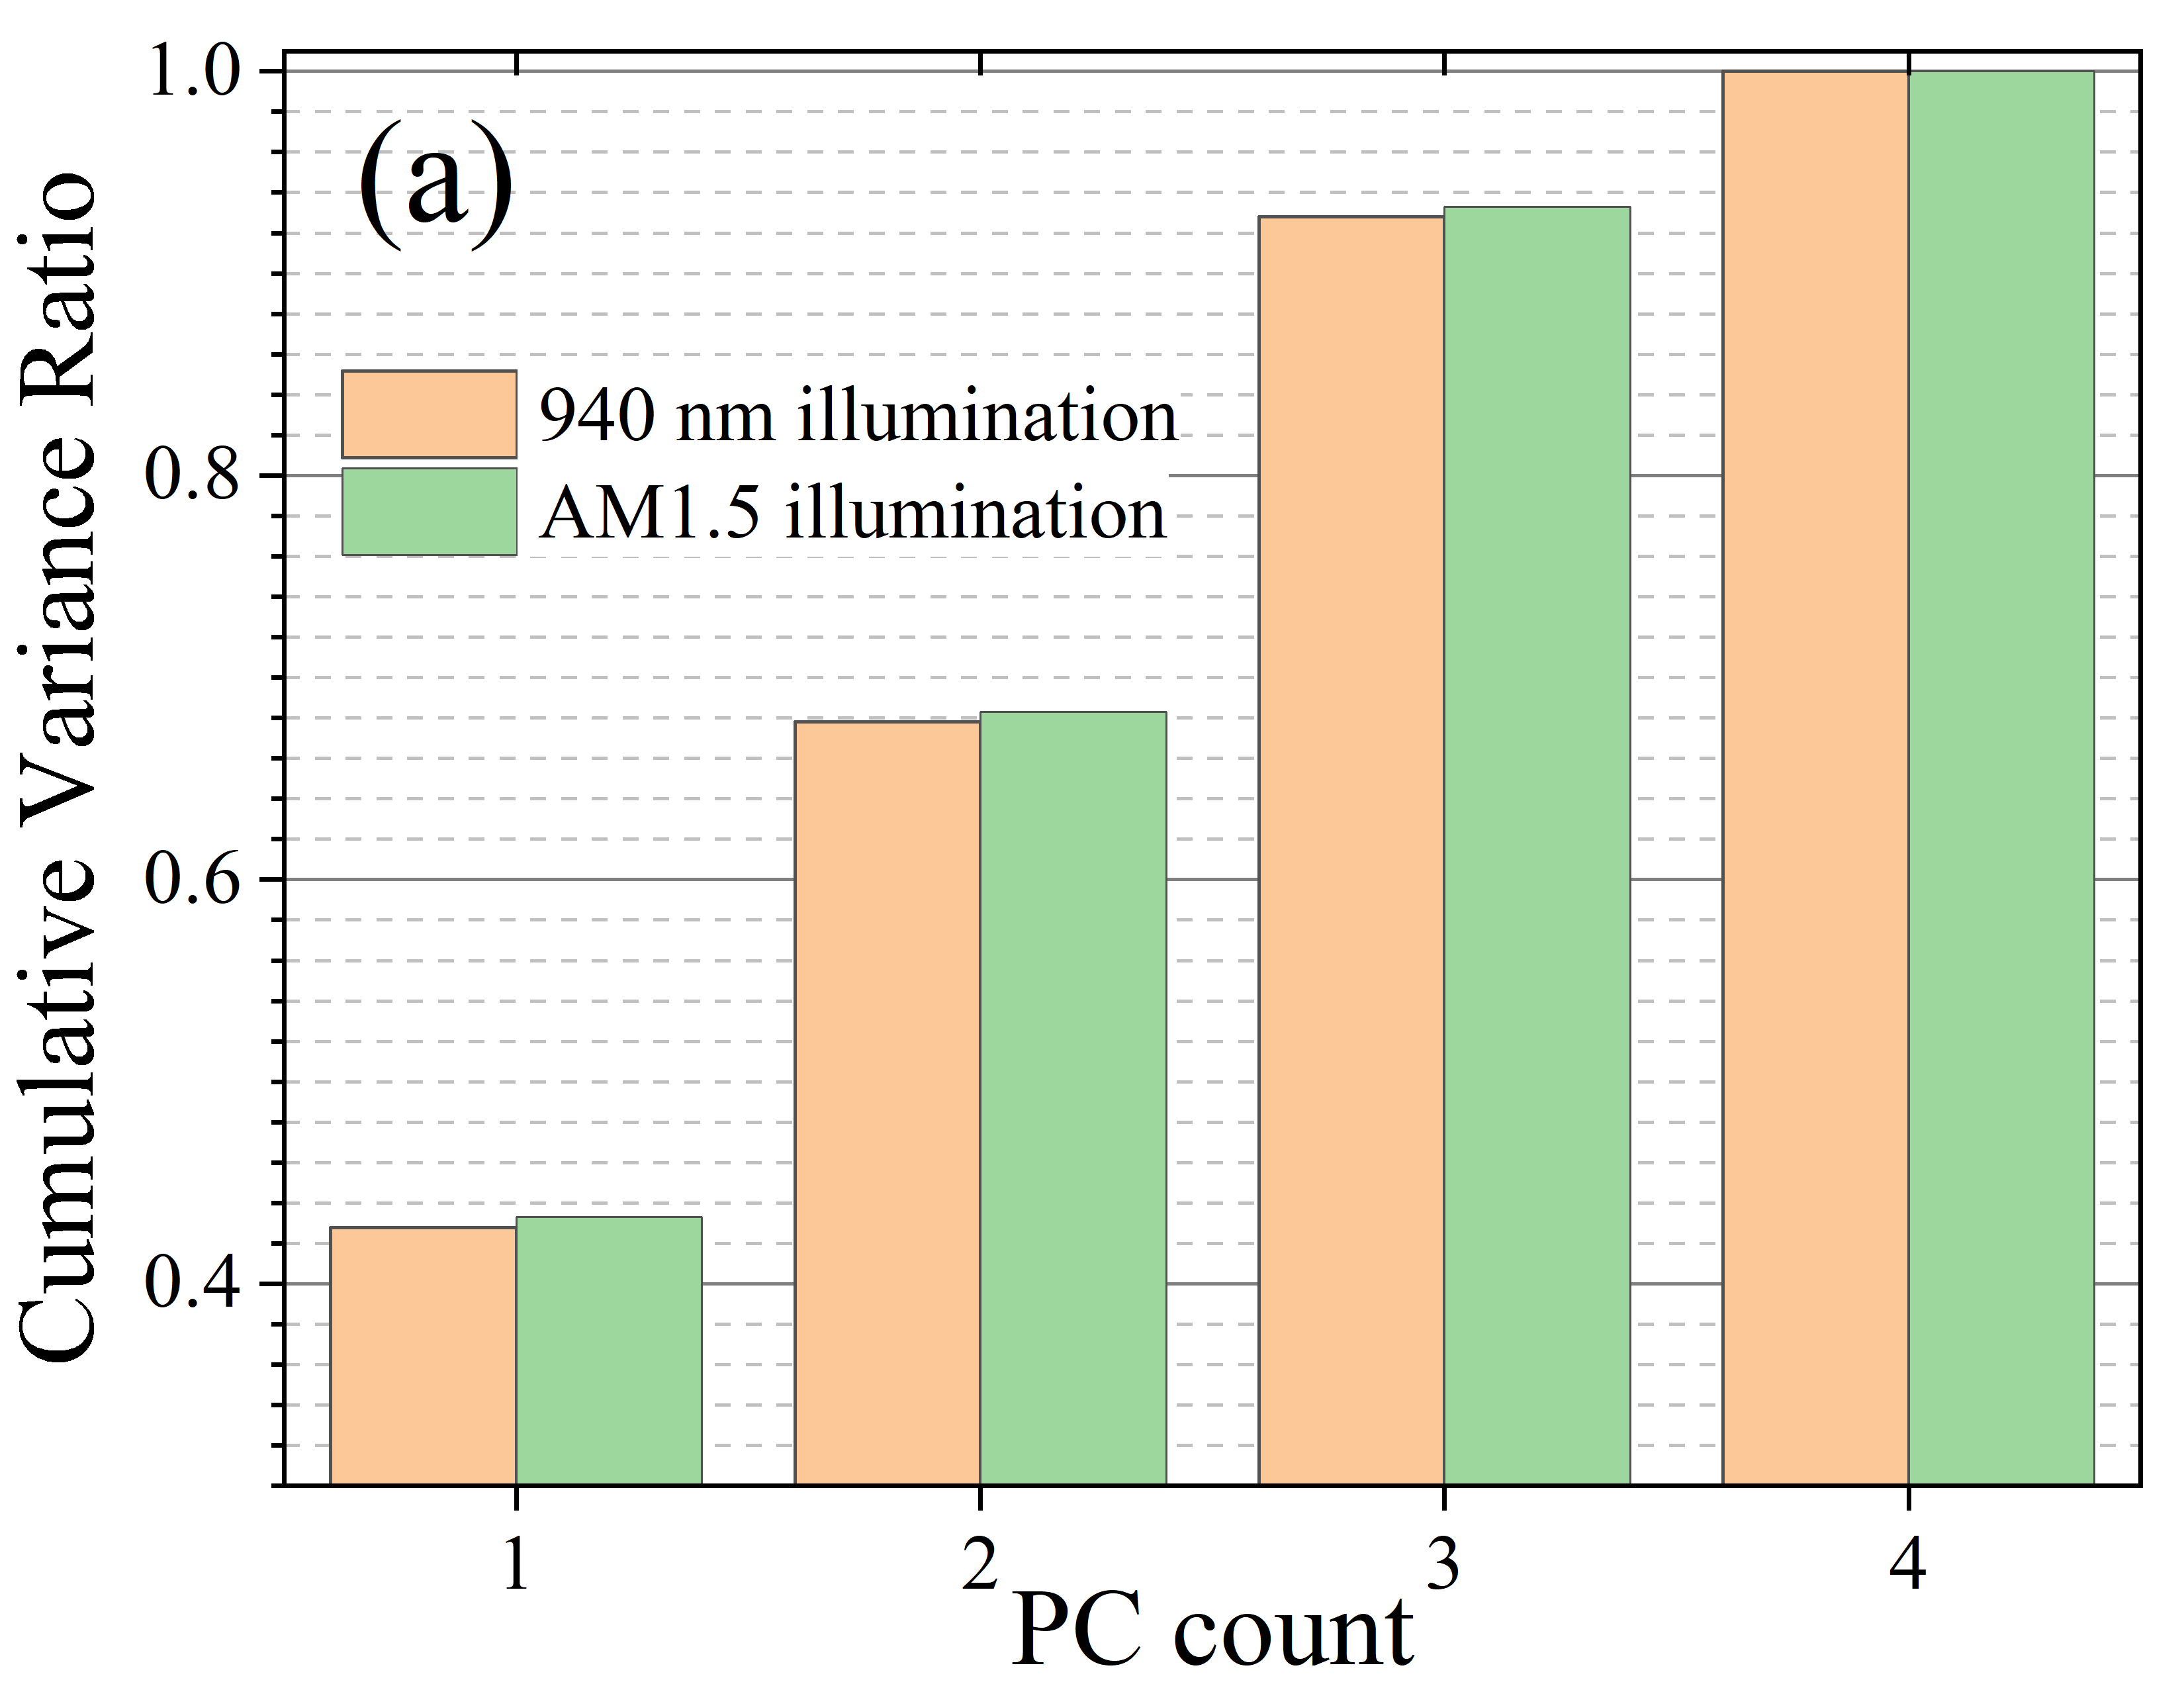
\includegraphics[width=0.4\linewidth]{Fig2a.png}
  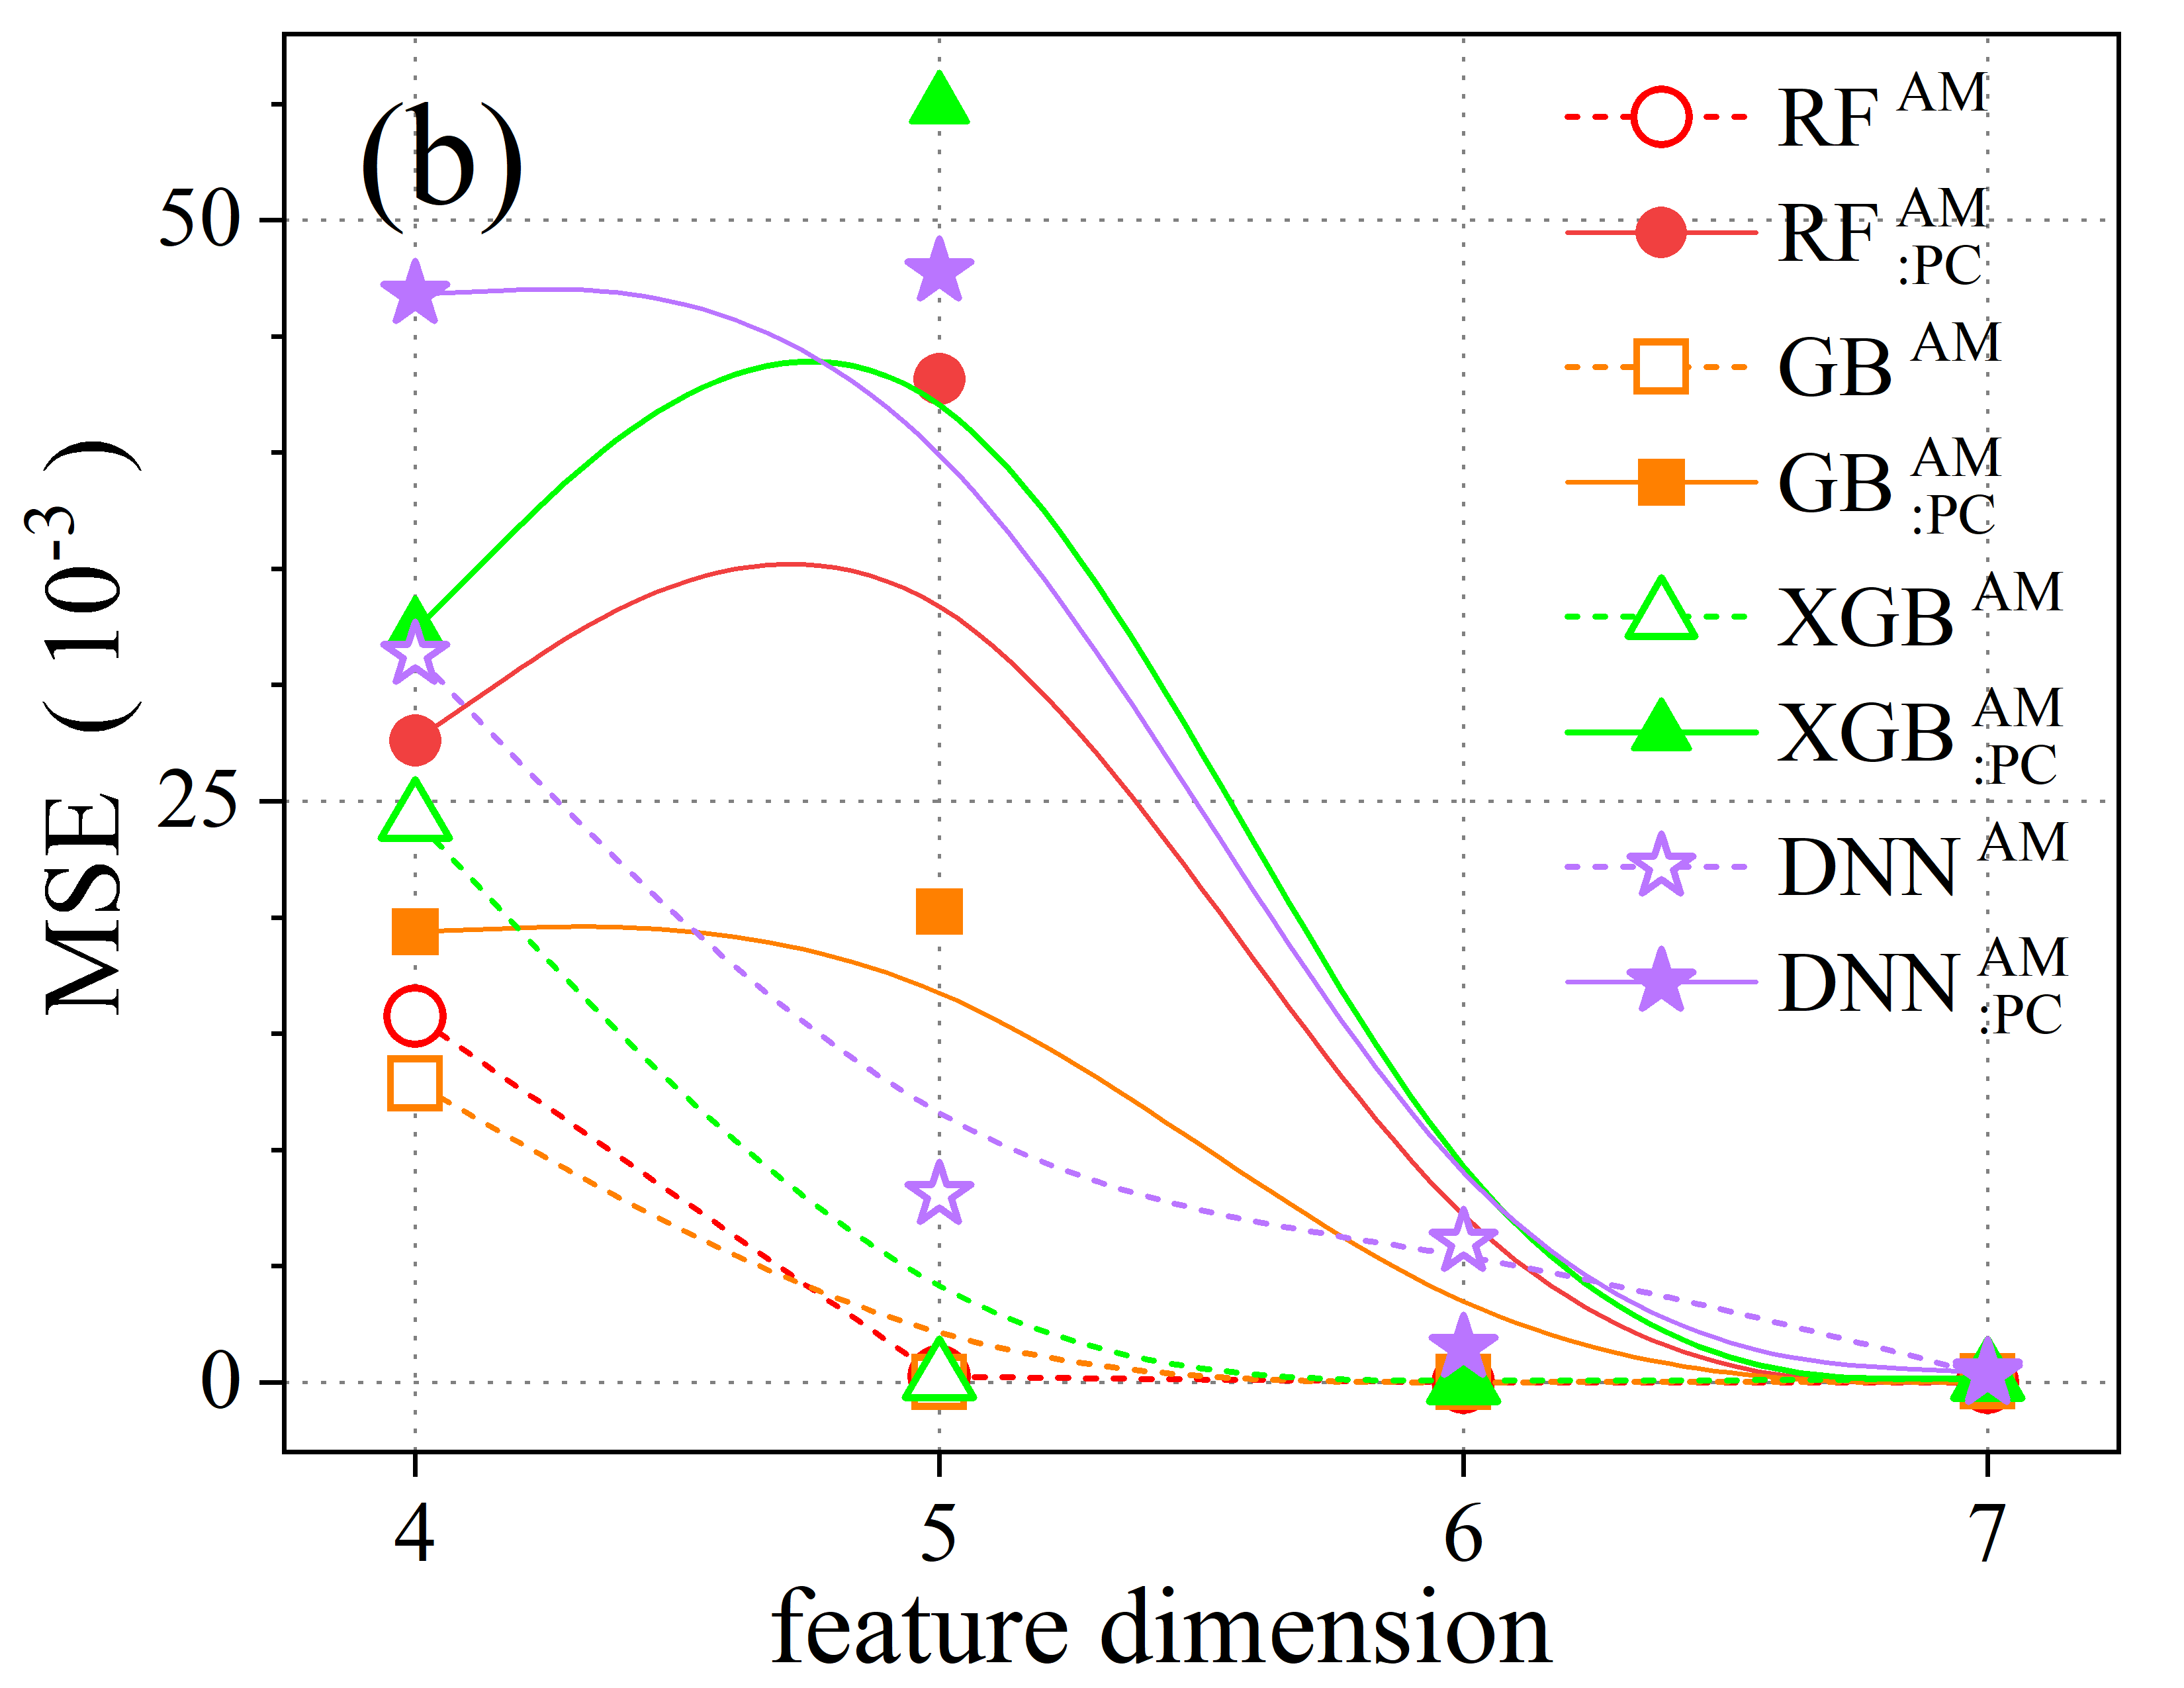
\includegraphics[width=0.4\linewidth]{Fig2b.png}
  \caption{Typical current-voltage characteristics measured
  under low-intensive LED illumination at 940~nm across different periods following exposure to strong light (halogen lamp) (panel a) and
  short circuit current plotted as a function of the time after high-intensive illumination (panel b).
  %The marks are the experimental results and the lines are given for convenience only (b) and the curves fitted according to \cite{Olikh2022:JMatSci,Olikh2021JAP}.
  The marks are the experimental results and the lines on panel b are the curves fitted according to \cite{Olikh2022:JMatSci,Olikh2021JAP}.
  Light sources: GE (a), Osram (b).
  $t_\mathrm{ill}$, s: 50 (a), 5(b).
  $W_\mathrm{ill}=400$~mW (a).
  $T=340$~K.}
  \label{fig2}
\end{figure}

\textbf{Figure~\ref{fig2}b} illustrates the dependencies $I_{SC}(t_\mathrm{dark})$ after illumination with different intensities.
As previously shown \cite{Olikh2021JAP}, the magnitude of the change in $I_{SC}$ after the dark recovery period
inherently correlates with the concentration of Fe$_i$ formed as a result of light-induced dissociation of FeB pairs.
From examining the presented data, it is evident that escalating $W_\mathrm{ill}$ leads to an augmentation in the dissociation efficiency.
Concurrently, the recovery time remains insensitive to the illumination parameters, which conforms to expectations,
given that the latter is determined by $R_a$ --- see Equation~(\ref{eqNFet}).

It should be noted that besides $N_\mathrm{Fe,0}$ values,
the fitting of short-circuit current \cite{Olikh2022:JMatSci,Olikh2021JAP} allows for the estimation of the energy of Fe$_i$ migration $E_m$
and bulk lifetime $\tau_\mathrm{other}$, which arises from recombination channels other than Fe-related defects and intrinsic recombination.
The obtained value $E_m=(0.650\pm0.005)$~eV coincides with that wellknown value \cite{FeBKin2019,FeBAssSST2011,FeBkinAPL2008}.
This coincidence confirms that the investigated processes are indeed associated with rebuilding,
as described by Equation~(\ref{eqReac}).
In turn, the value of $E_m$ allows for the estimation of the recombination rate \cite{FeBAssJAP2014,FeBKin2019,FeBAssSST2011}:
\begin{equation}
\label{eqTass}
R_a^{-1}=5.7\times10^5\,\frac{\mathrm{s}}{\mathrm{K}\;\mathrm{cm}^3}\times\frac{T}{p}\exp\left(\frac{E_m}{kT}\right)\,.
\end{equation}
Thus, in our case, $R_a=(1.68\pm0.03)\times10^{-3}$~s$^{-1}$.

Regarding the value of $\tau_\mathrm{other}$, it was found to significantly exceed the
lifetime associated with Shockley-Read–Hall (SRH) recombination on Fe-related defects (about $2.2$~$\mu$m).
Notably, according M\"{o}ller~\emph{et al.} \cite{FeBAssJAP2014},
such a condition is essential for the accurate determination of the constant $K$, which is included in Equation~(\ref{eqRd}).


The dependencies of the concentration of interstitial atoms on illumination time are shown in \textbf{Figure~\ref{fig3}}.
From the data, it's evident that the pair dissociation rate is significantly influenced by the illumination intensity.
This effect is consistent across all utilized light sources.
Nonetheless, the $W_\mathrm{ill}$ value is not the exclusive determining factor for the pair dissociation rate,
as demonstrated in Figure~\ref{fig3}d.
For instance, when using the GE source, pair dissociation occurs most efficiently.
With Osram, the process unfolds more slowly,
and illumination with Orion, under otherwise identical conditions, proves to be the least effective in terms of altering the state of FeB pairs.


\begin{figure}
\centering
  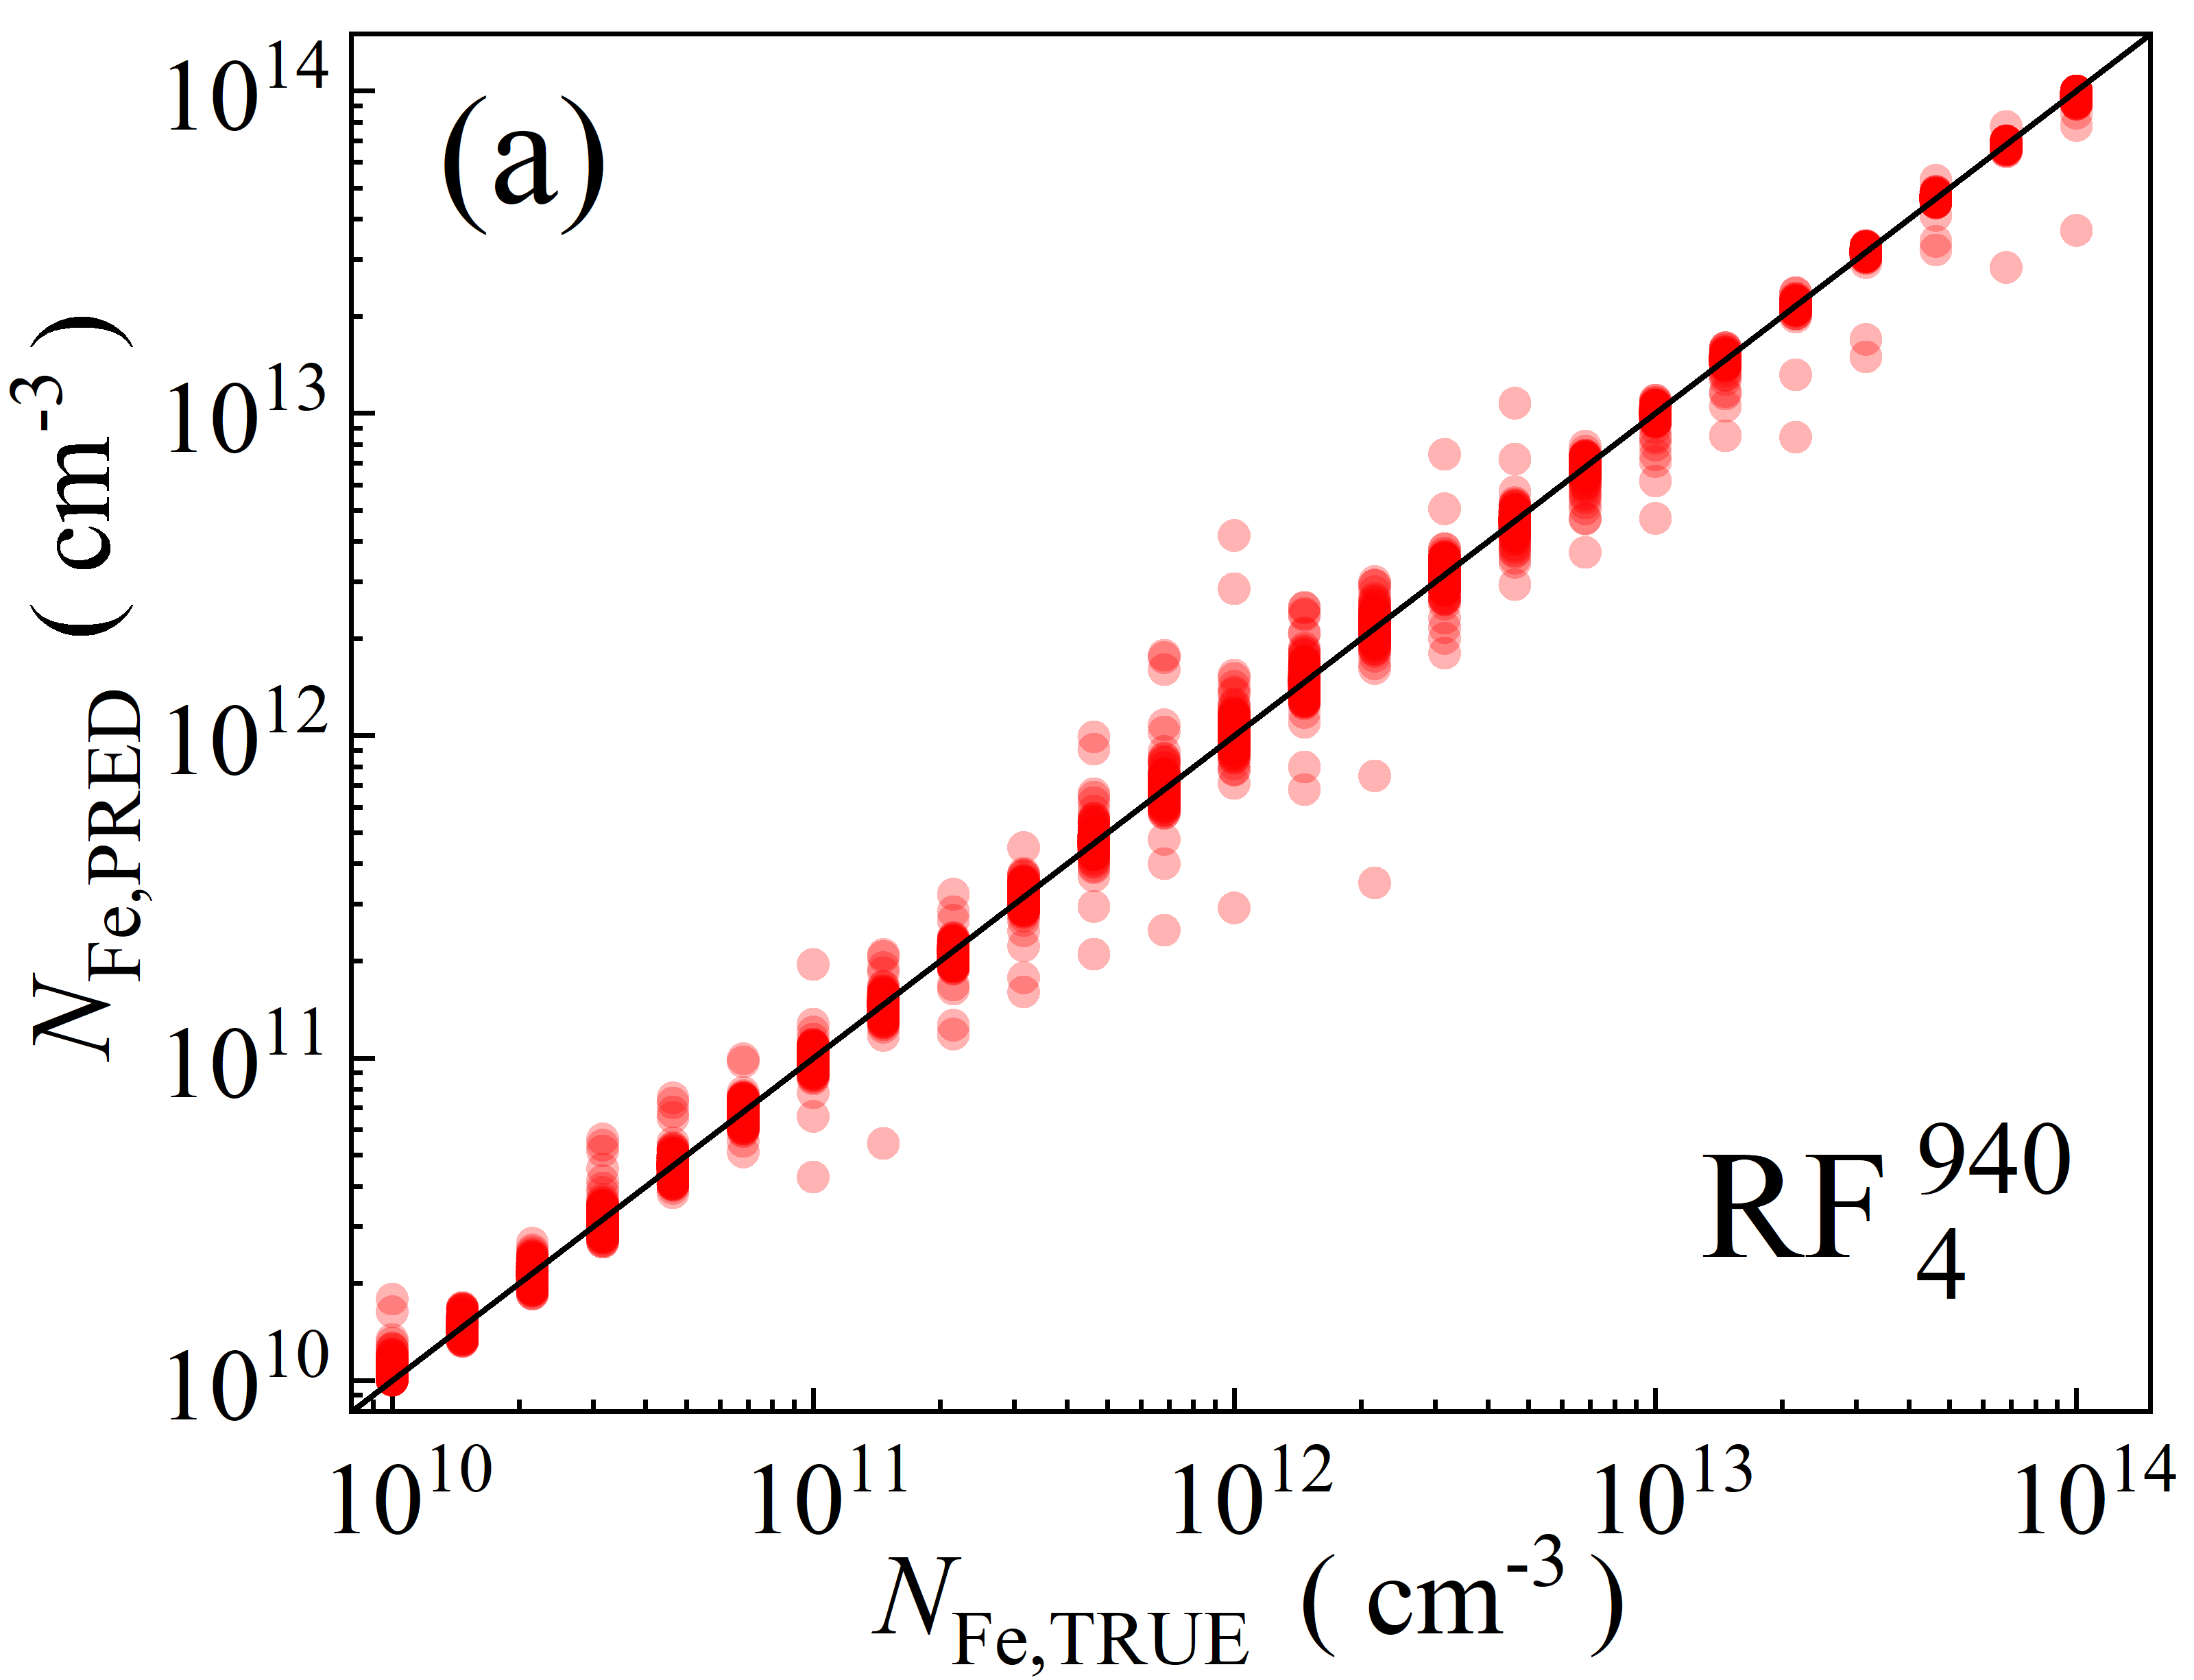
\includegraphics[width=0.4\linewidth]{Fig3a.png}
  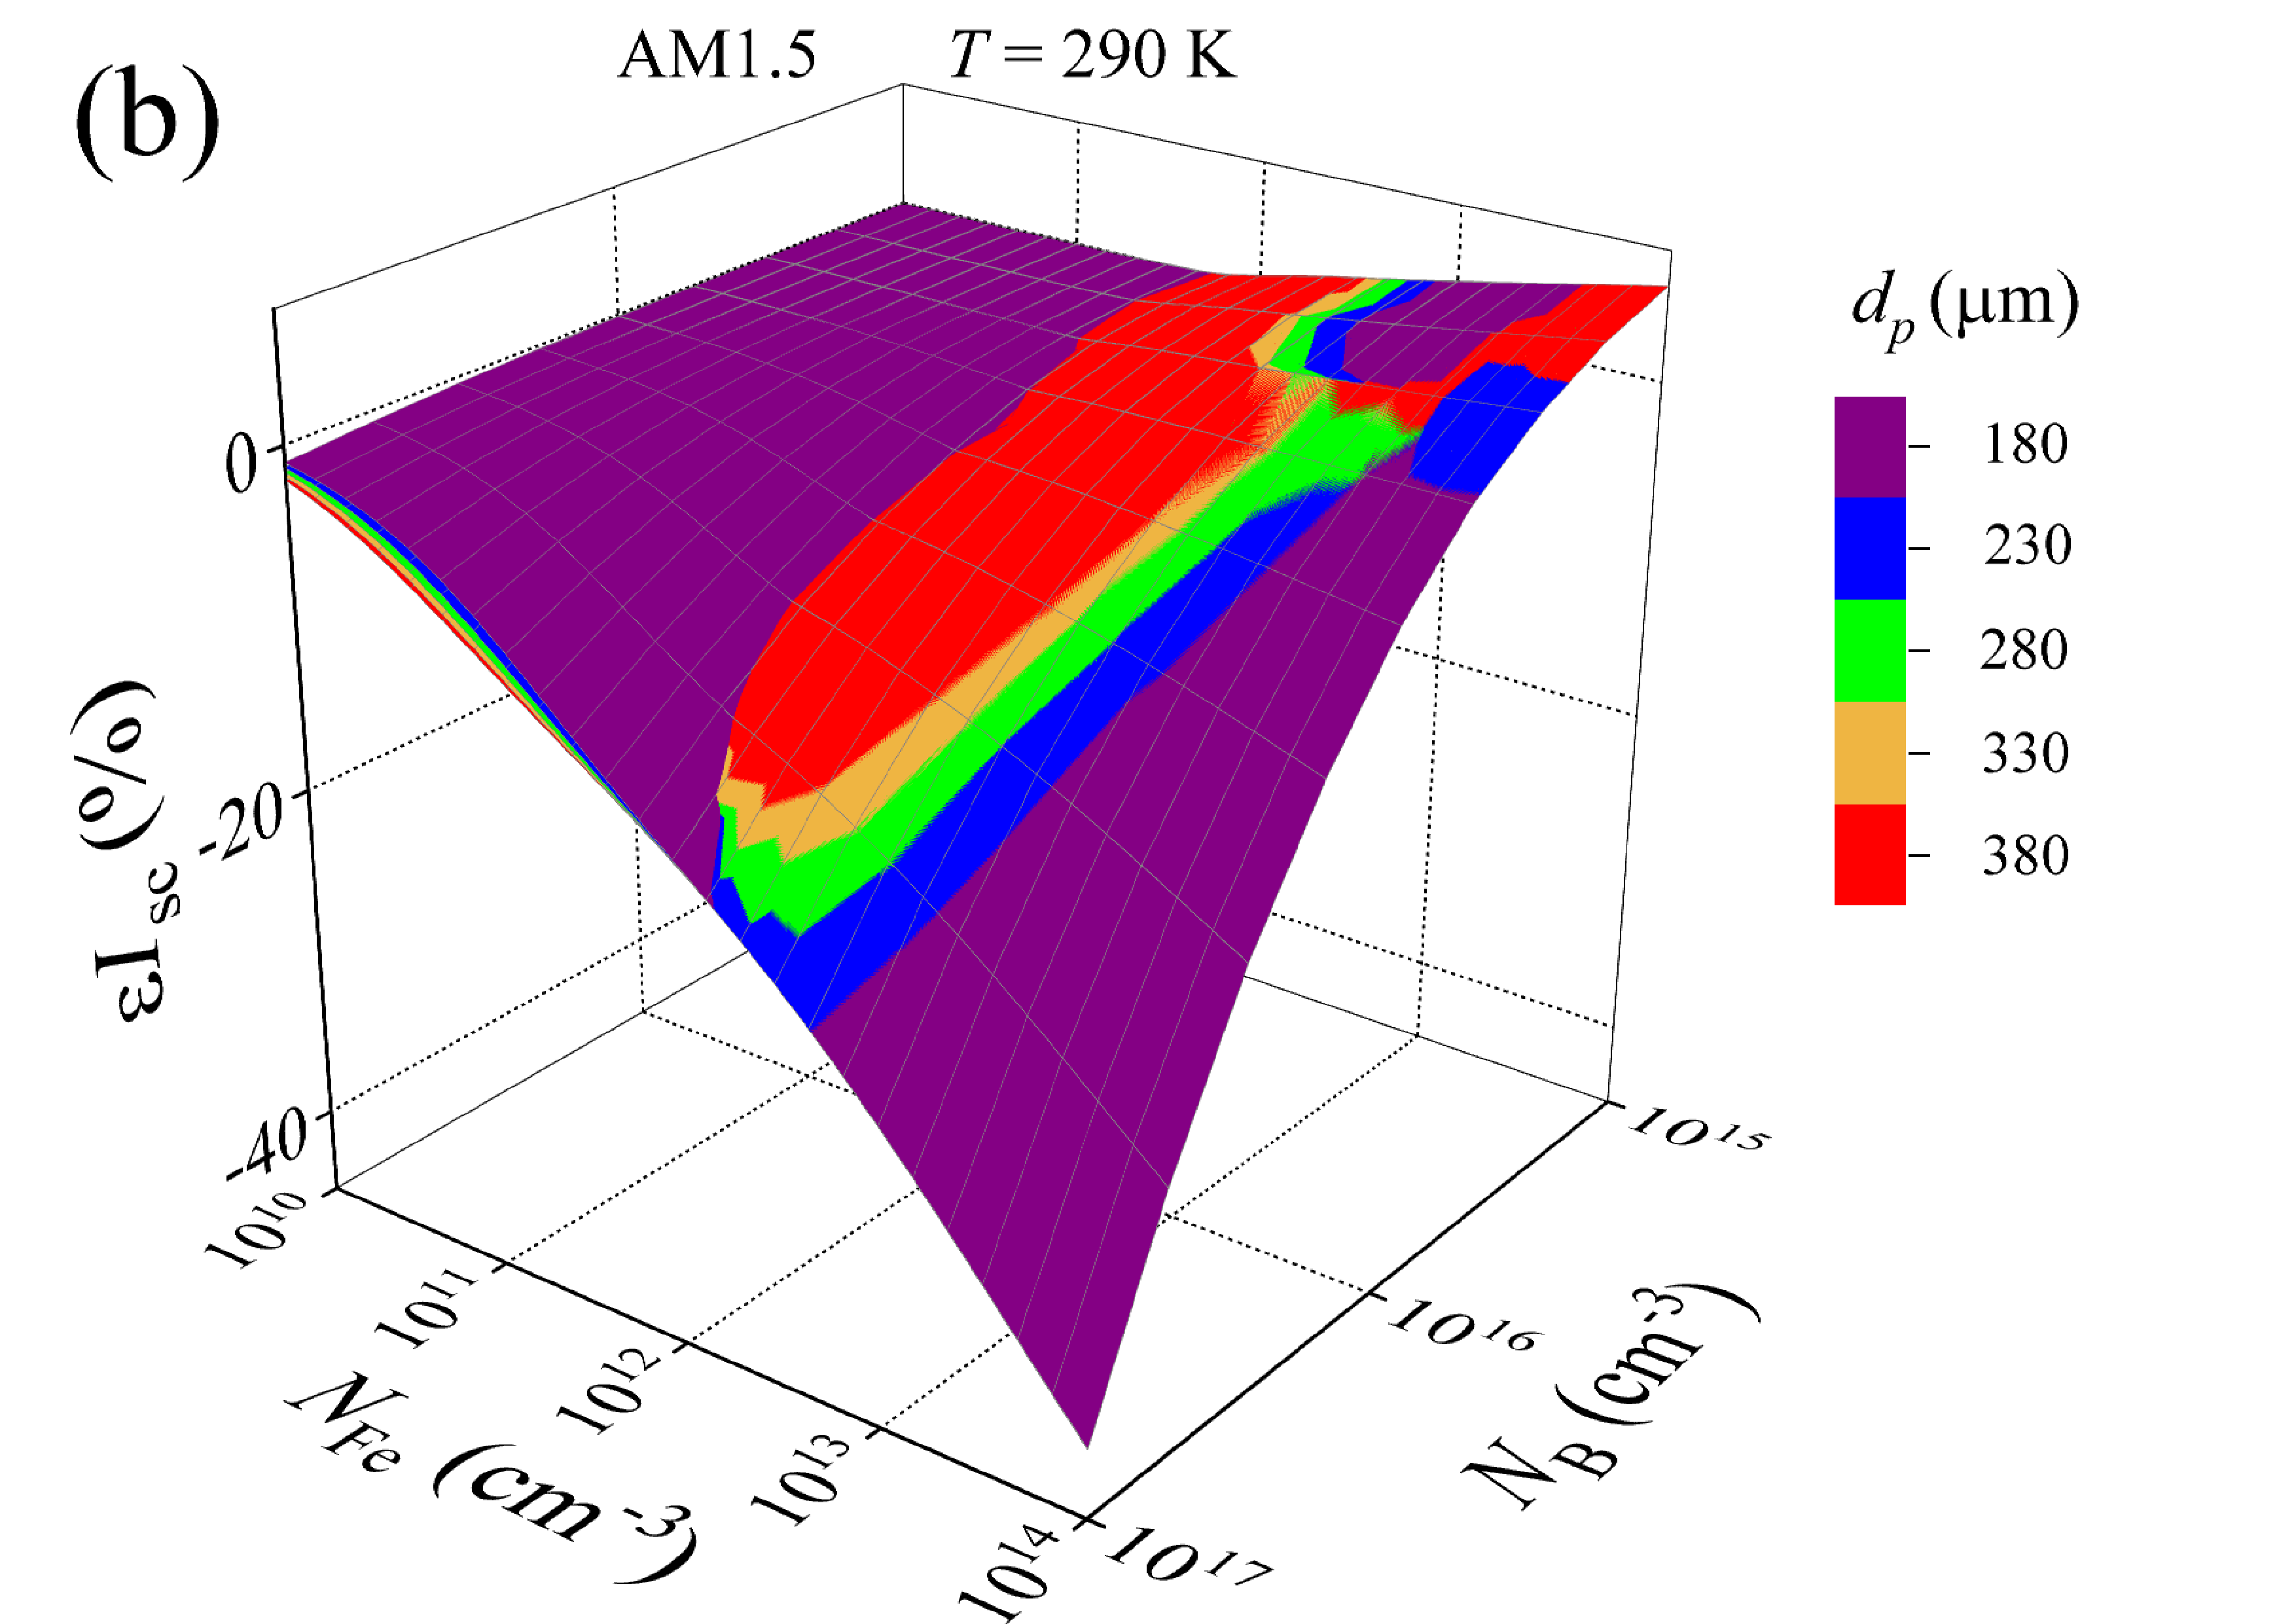
\includegraphics[width=0.4\linewidth]{Fig3b.png}
  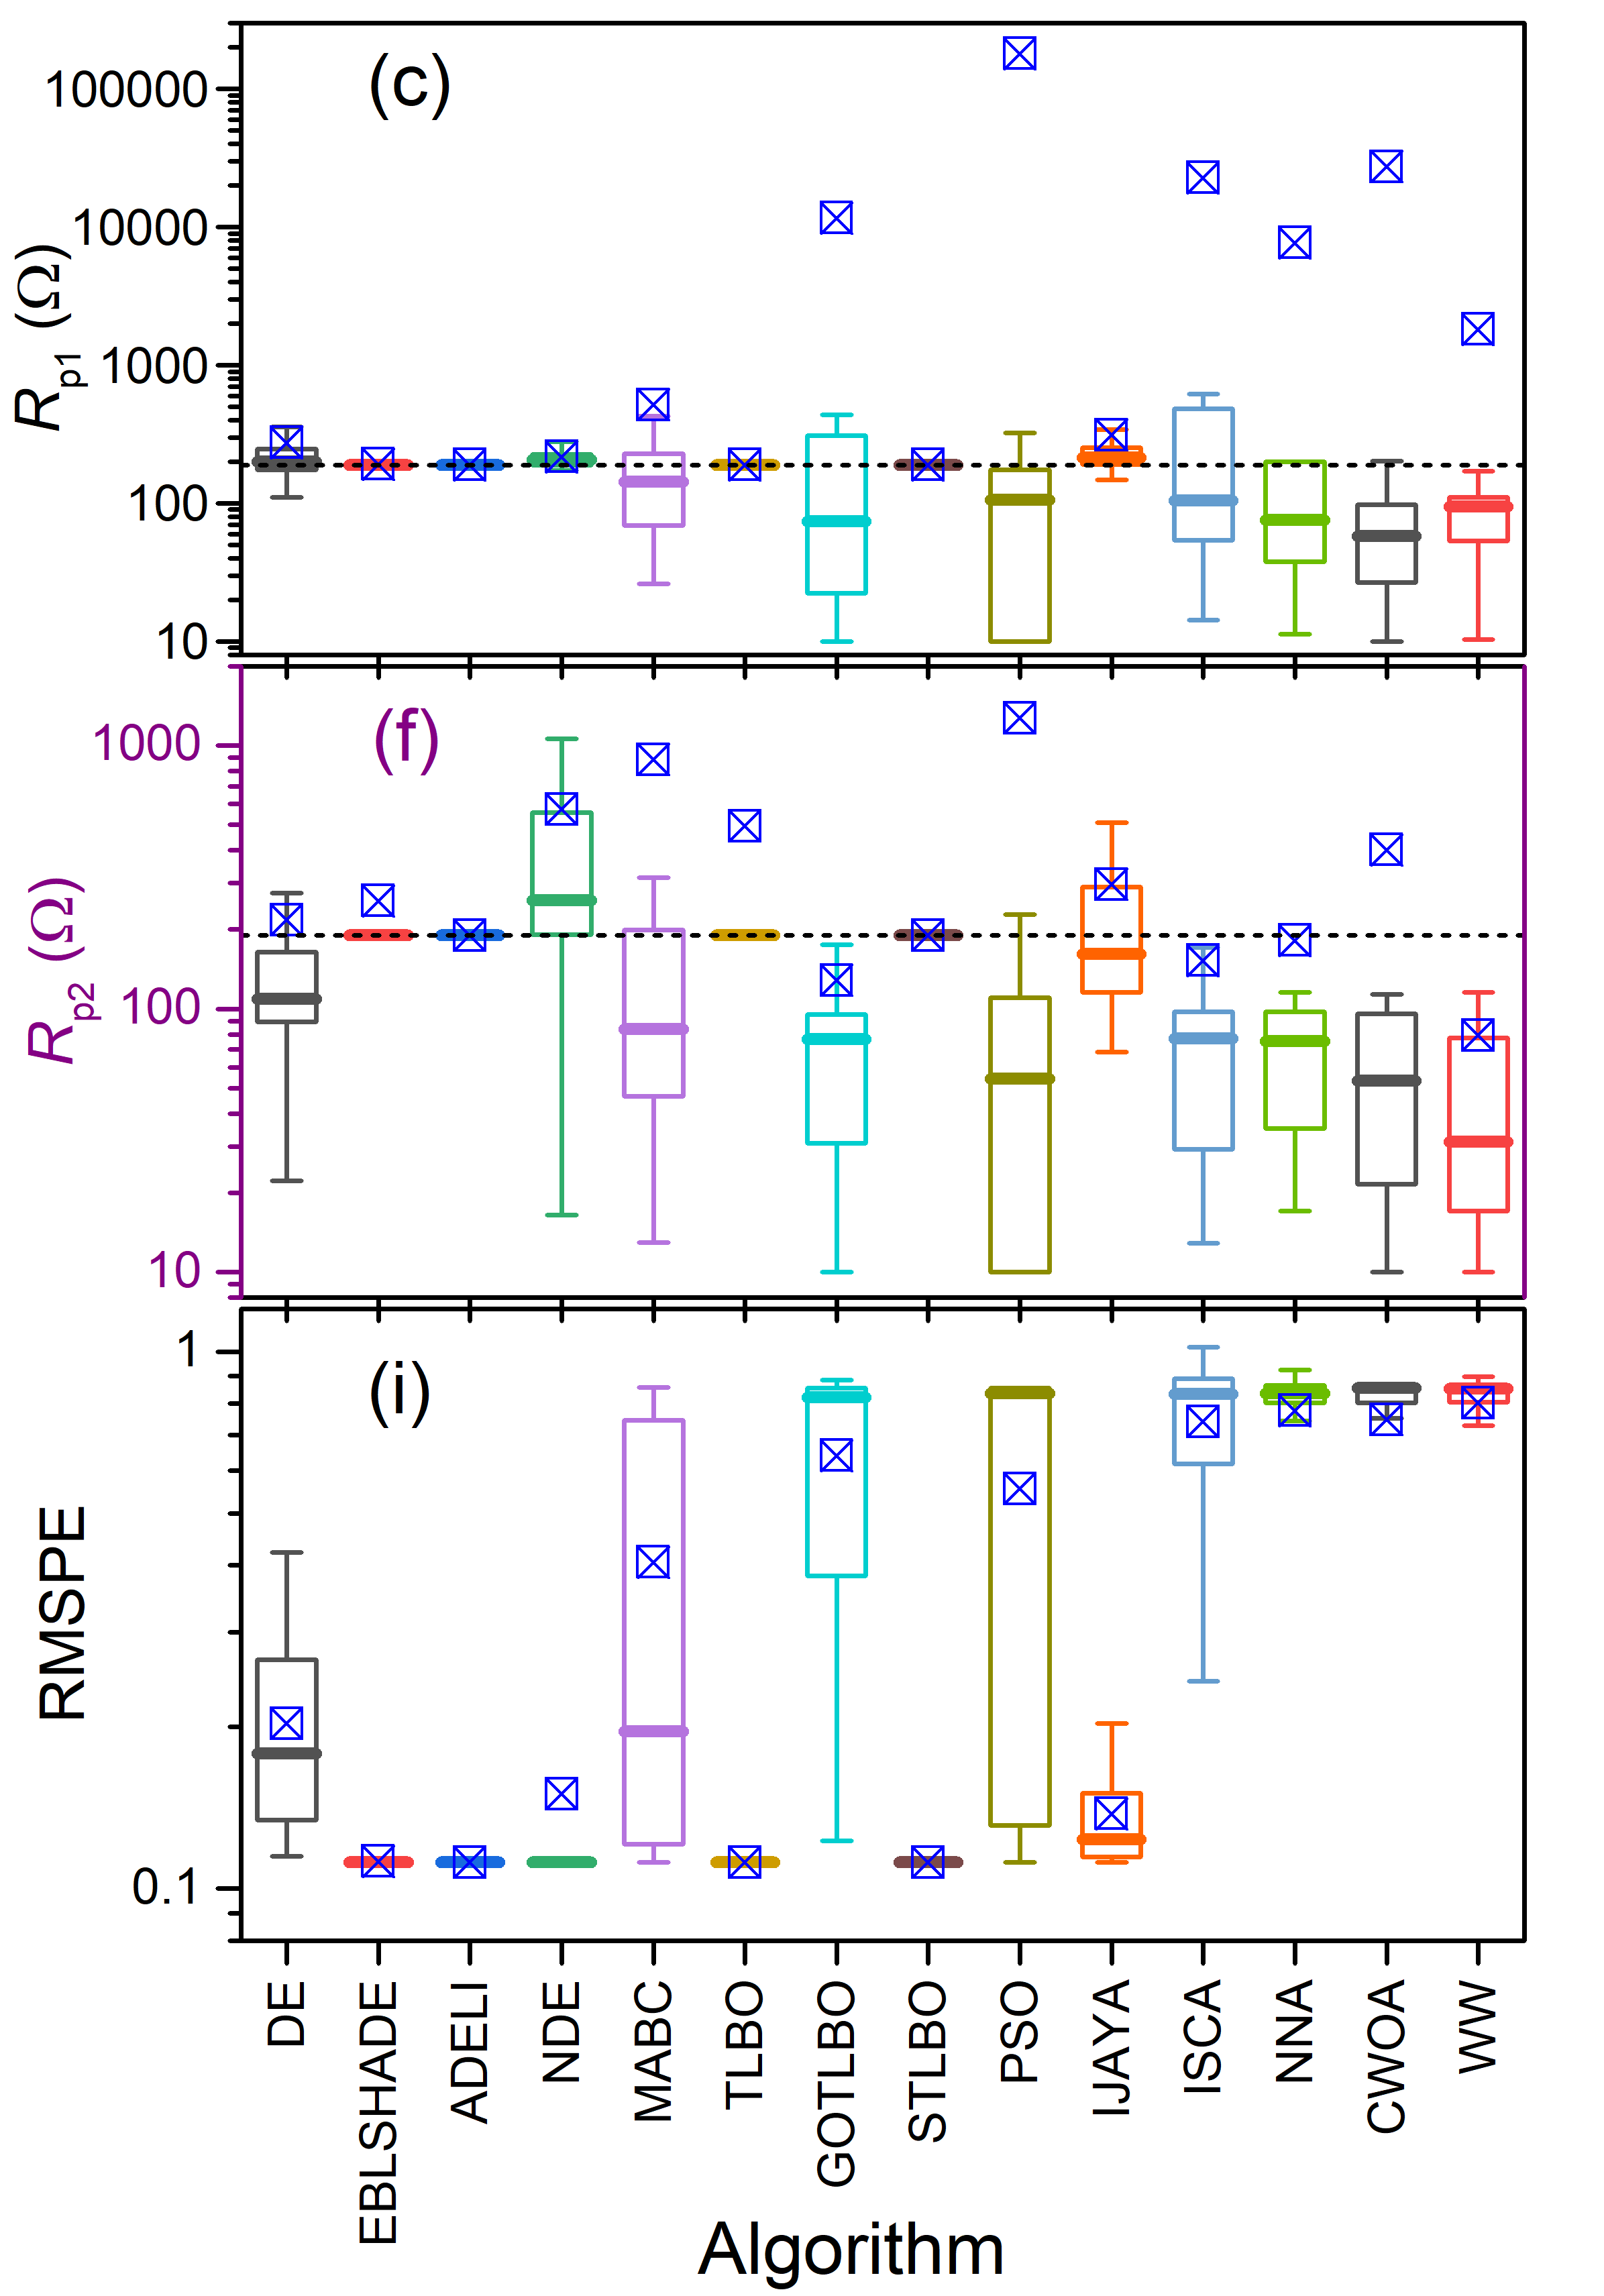
\includegraphics[width=0.4\linewidth]{Fig3c.png}
  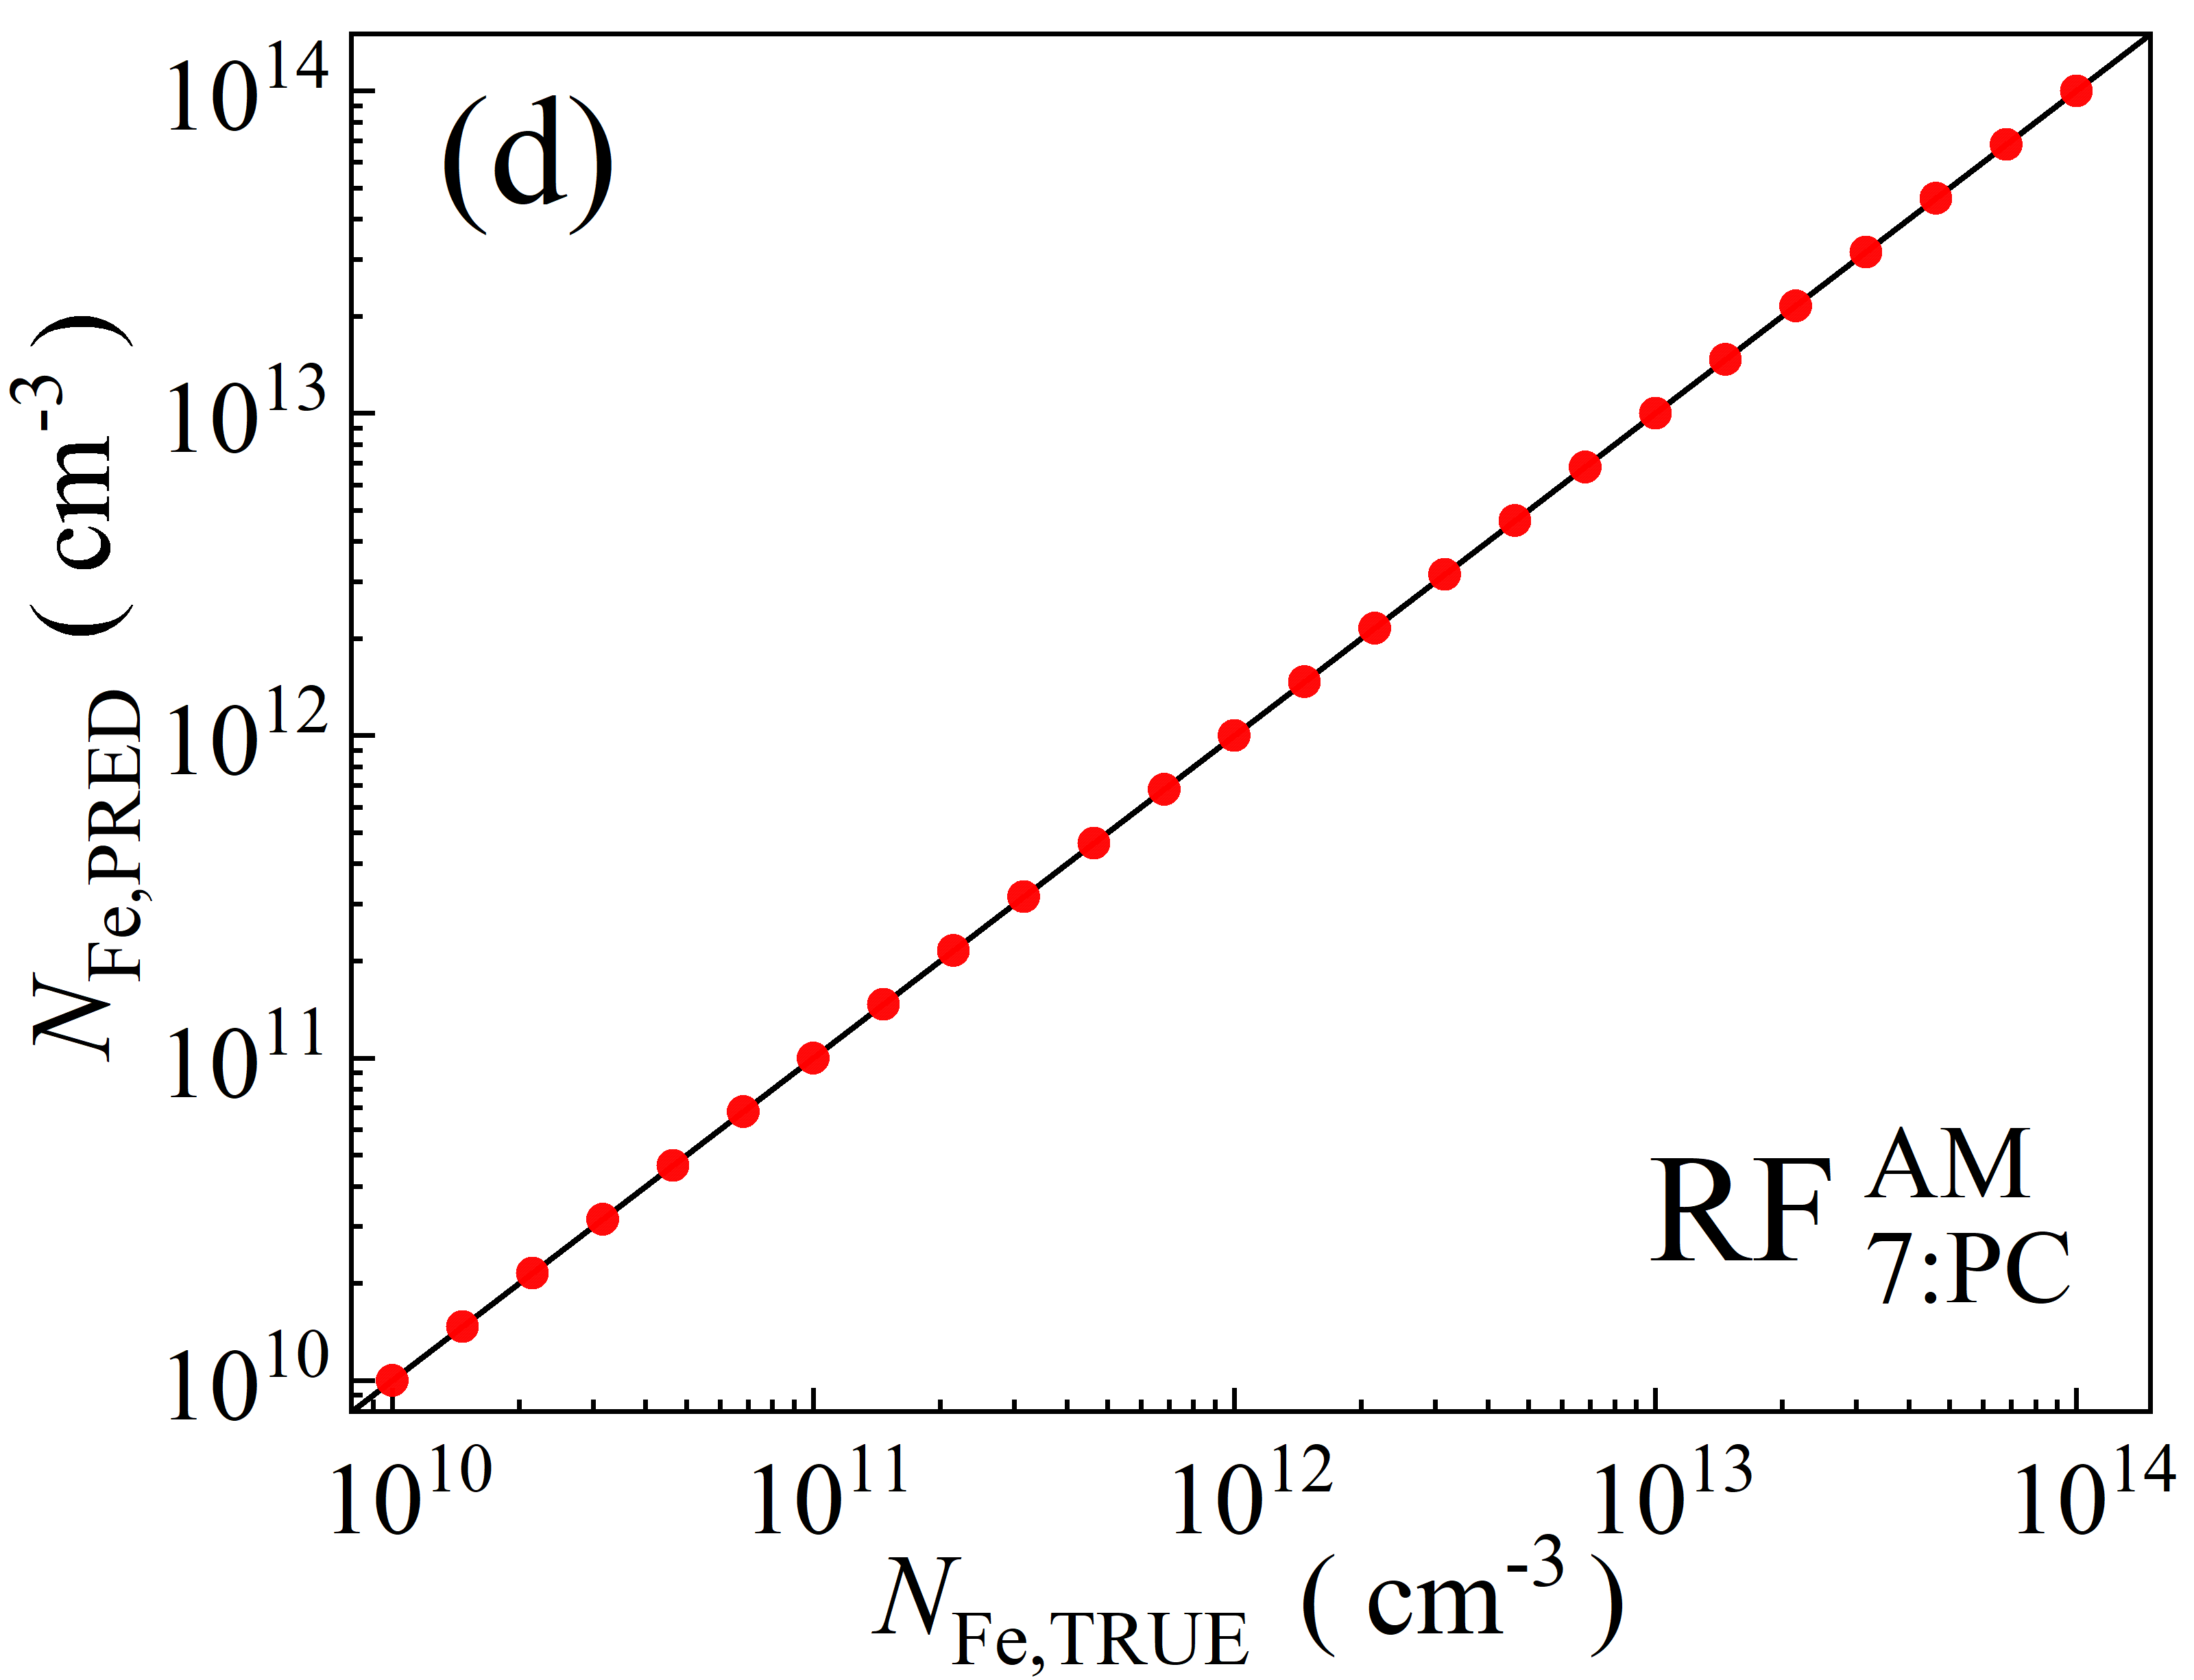
\includegraphics[width=0.4\linewidth]{Fig3d.png}
  \caption{The relationships between the concentration of FeB pairs following intense illuminations of varying intensities and the illumination duration.
  Light source: Orion (a), Osram (b), GE (c).
  Panel d highlights variations in the dissociation of pairs induced by different light sources.
  The marks are the experimental results, the lines are the fitted curves using Equation~(\ref{eqNfe0Exp}).
  $T=340$~K.}
  \label{fig3}
\end{figure}


The experimentally obtained dependencies $N_\mathrm{Fe,0}(t_\mathrm{ill})$ were fitted using the equation
\begin{equation}
\label{eqNfe0Exp}
N_\mathrm{Fe,0}(t_\mathrm{ill})=A\exp(-t_\mathrm{ill}/\tau_\mathrm{dis})
+N_\mathrm{Fe,fit}\,,
\end{equation}
where
$\tau_\mathrm{dis}$ is the characteristic dissociation time,
and $N_\mathrm{Fe,fit}$ concentration of dissociated pairs at saturation.
The fitting results, shown in Figure~\ref{fig3} as lines and listed in the \textbf{Table~\ref{tb1}},
include the coefficients of determination $R^2$.
The high values of $R^2$ (greater than 0.99) confirm the suitability of the chosen approximation formula.


\begin{table}
 \caption{ Fitting results of experimental dependencies $N_\mathrm{Fe,0}(t_\mathrm{ill})$
 using Equation~(\ref{eqNfe0Exp}) and defect parameter estimation using Equations~(\ref{eqTauRd}-\ref{eqFefit}).
% The value of maximum concentrations of iron atoms after illumination and
%characteristic dissociation time obtained by fitting experimental dependencies by Equation~(\ref{eqNfe0Exp}).
%Coefficient of determination is listed as well.
}
 \label{tb1}
  \begin{tabular}[htbp]{@{}ccccccc@{}}
    \hline
    $W_\mathrm{ill}$~[mW] & Light source & \multicolumn{3}{c}{fitting parameters}&\multicolumn{2}{c}{defect parameters} \\
     &  & $\tau_\mathrm{dis}$ [s] & $N_\mathrm{Fe,fit}$ [$10^{12}$~cm$^3$] & $R^2$ & $R_d$ [$10^{-3}$~s$^{-1}$] & $N_\mathrm{Fe,tot}$ [$10^{12}$~cm$^{-3}$] \\
    \hline
    750  & Orion  & $2.2\pm0.2$ & $8.6\pm0.1$ & 0.993 &450&8.6\\
    700  & Orion  & $2.7\pm0.2$ & $8.7\pm0.1$ & 0.995 &370&8.7\\
         & Osram  & $2.4\pm0.2$ & $8.6\pm0.1$ & 0.992 &410&8.6\\
    600  & Orion  & $3.7\pm0.2$ & $8.65\pm0.06$ & 0.998&270&8.7 \\
         & Osram  & $3.0\pm0.2$ & $8.69\pm0.08$ & 0.995&330&8.7 \\
    500  & Orion  & $5.5\pm0.2$ & $8.65\pm0.04$ & 0.999&180&8.7 \\
         & Osram  & $4.5\pm0.1$ & $8.7\pm0.1$ & 0.998&220&8.8 \\
    400  & Orion  & $8.8\pm0.3$ & $8.74\pm0.06$ & 0.998&110&8.8 \\
         & Osram  & $6.1\pm0.2$ & $8.63\pm0.08$ & 0.997 &160&8.7\\
         & GE  & $3.6\pm0.3$ & $8.7\pm0.1$ & 0.996 &280&8.7\\
    300  & Orion  & $15.7\pm0.6$ & $8.6\pm0.1$ & 0.998 &62&8.8\\
         & Osram  & $12.4\pm0.1$ & $8.69\pm0.02$ & 0.999&79&8.8 \\
         & GE  & $6.5\pm0.2$ & $8.69\pm0.05$ & 0.998 &150&8.8\\
    200  & Orion  & $35\pm3$ & $8.5\pm0.3$ & 0.998 &27&8.8\\
         & Osram  & $24\pm1$ & $8.6\pm0.1$ & 0.999 &40&8.9\\
         & GE  & $15.1\pm0.5$ & $8.7\pm0.1$ & 0.999 &65&8.8\\
    \hline
  \end{tabular}
\end{table}




The comparison of Equations~(\ref{eqNfeill}) and (\ref{eqNfe0Exp}) reveals a relationship between
the fitting parameters and defect characteristics, specifically:
\begin{equation}
\label{eqTauRd}
\tau_\mathrm{dis}^{-1}=R_a+R_d\,,
\end{equation}
\begin{equation}
\label{eqFefit}
N_\mathrm{Fe,fit}=N_\mathrm{Fe,tot}\frac{R_d}{R_d+R_a}\,.
\end{equation}

%\begin{eqnarray}
%\label{eqTauRd}
%\tau_\mathrm{dis}^{-1}&=&R_a+R_d\,,\\
%\label{eqFefit}
%N_\mathrm{Fe,fit}&=&N_\mathrm{Fe,tot}\frac{R_d}{R_d+R_a}\,.
%%A&=&N_\mathrm{Fe,eq}-N_\mathrm{Fe,tot}\frac{R_d}{R_d+R_a}\,.
%\end{eqnarray}

The fitting parameters and recombination rate of  $1.68\times10^{-3}$~s obtained 
were used to calculate the $N_\mathrm{Fe,tot}$ and $R_d$ values listed in the Table~\ref{tb1}.
Data suggest that regardless of the light source used and $W_\mathrm{ill}$,
the observed total concentration of impurity iron atom is consistently
$N_\mathrm{Fe,tot}=(8.7\pm0.1)\times10^{12}$~cm$^{-3}$.
This stability supports the accuracy of the analysis.
However, the FeB dissociation rate may vary significantly for the same intensity value depending on the light source used.

According to Wijaranakula \cite{FeB:kinetic}, at the specified value of $N_\mathrm{Fe,tot}$,
the equilibrium (in darkness) concentrations of interstitial iron atoms $N_\mathrm{Fe,eq}$ and FeB pairs
$N_\mathrm{FeB}$ at $T=340$~K are $1.3\times10^{12}$~cm$^{-3}$ and $7.4\times10^{12}$~cm$^{-3}$, respectively.
The values of $N_\mathrm{Fe,eq}$ and $N_\mathrm{FeB}$ were used to estimate the minority carrier diffusion length $L_n$
in the base of the used solar cell.
It was assumed that the dominant recombination processes are SRH recombination at Fe$_i$ and FeB and intrinsic recombination.
The required electron mobility $\mu_n$ value were taken from Klaassen \cite{KLAASSEN953},
the capture cross sections and energy levels for Fe$_i$ and FeB from Rougieux \emph{et al.} \cite{ROUGIEUX2018},
the coefficients of band-to-band radiation recombination and Auger recombination from
Niewelt \emph{et al.} \cite{Brad2022} and Black \& Macdonald \cite{AugerSi2022}, respectively.
The calculated value was found to be $L_n=80$~$\mu$m,
which is remarkably close to the value of 86~$\mu$m  obtained from the study of temperature dependencies of short-circuit current --- see Supplementary materials.


\subsection{Carrier generation rate estimation}\label{SecG}

The dissociation rate of FeB pairs during light-induced decay is well known
to be dependent on the carrier generation rate --- see Equation~(\ref{eqRd}).
Our subsequent objective involved determining the values of $G$ for various light sources.
The measured dependencies of spectral intensity $w_\mathrm{ill}$ of illumination incident on the sample under diverse conditions
are shown in \textbf{Figure~\ref{fig4}}.
It is crucial to highlight that our focus is specifically on the light reaching the sample;
hence, the spectrum is altered not only by the infrared transparency of the lamp reflector but also by absorption in the fiber
utilized to transmit the light flux to the solar cell.
Analogous modifications to the illumination spectra have been observed previously \cite{Libra2017}.
Figure~\ref{fig4}a displays discrepancies in the illumination spectra obtained from different light sources,
attributed to variations in the operational temperatures of the halogen lamps and differences in reflectors
(photos of the lamps are in the inset of Figure~\ref{fig4}a).
It is important to note that the upper limit of the spectra in Fig~\ref{fig4} (1120~nm)
is limited by the silicon bandgap, which, according to Passler \cite{Pasler}, corresponds to 1.11~eV at 340 K.
Furthermore, Figure~\ref{fig4}b demonstrates the change in the Osram spectrum with integral intensity increasing.
Notably, in addition to the expected increase in the curve's area, a minor spectrum shift towards shorter wavelengths is observed.
These behaviour is typical for all used light sources.

%A part of the radiation especially in the near infrared region of the spectrum is modified by infrared transparency of the reflector and by absorption in
%the plexiglass window. \cite{Libra2017}


\begin{figure}
\centering
  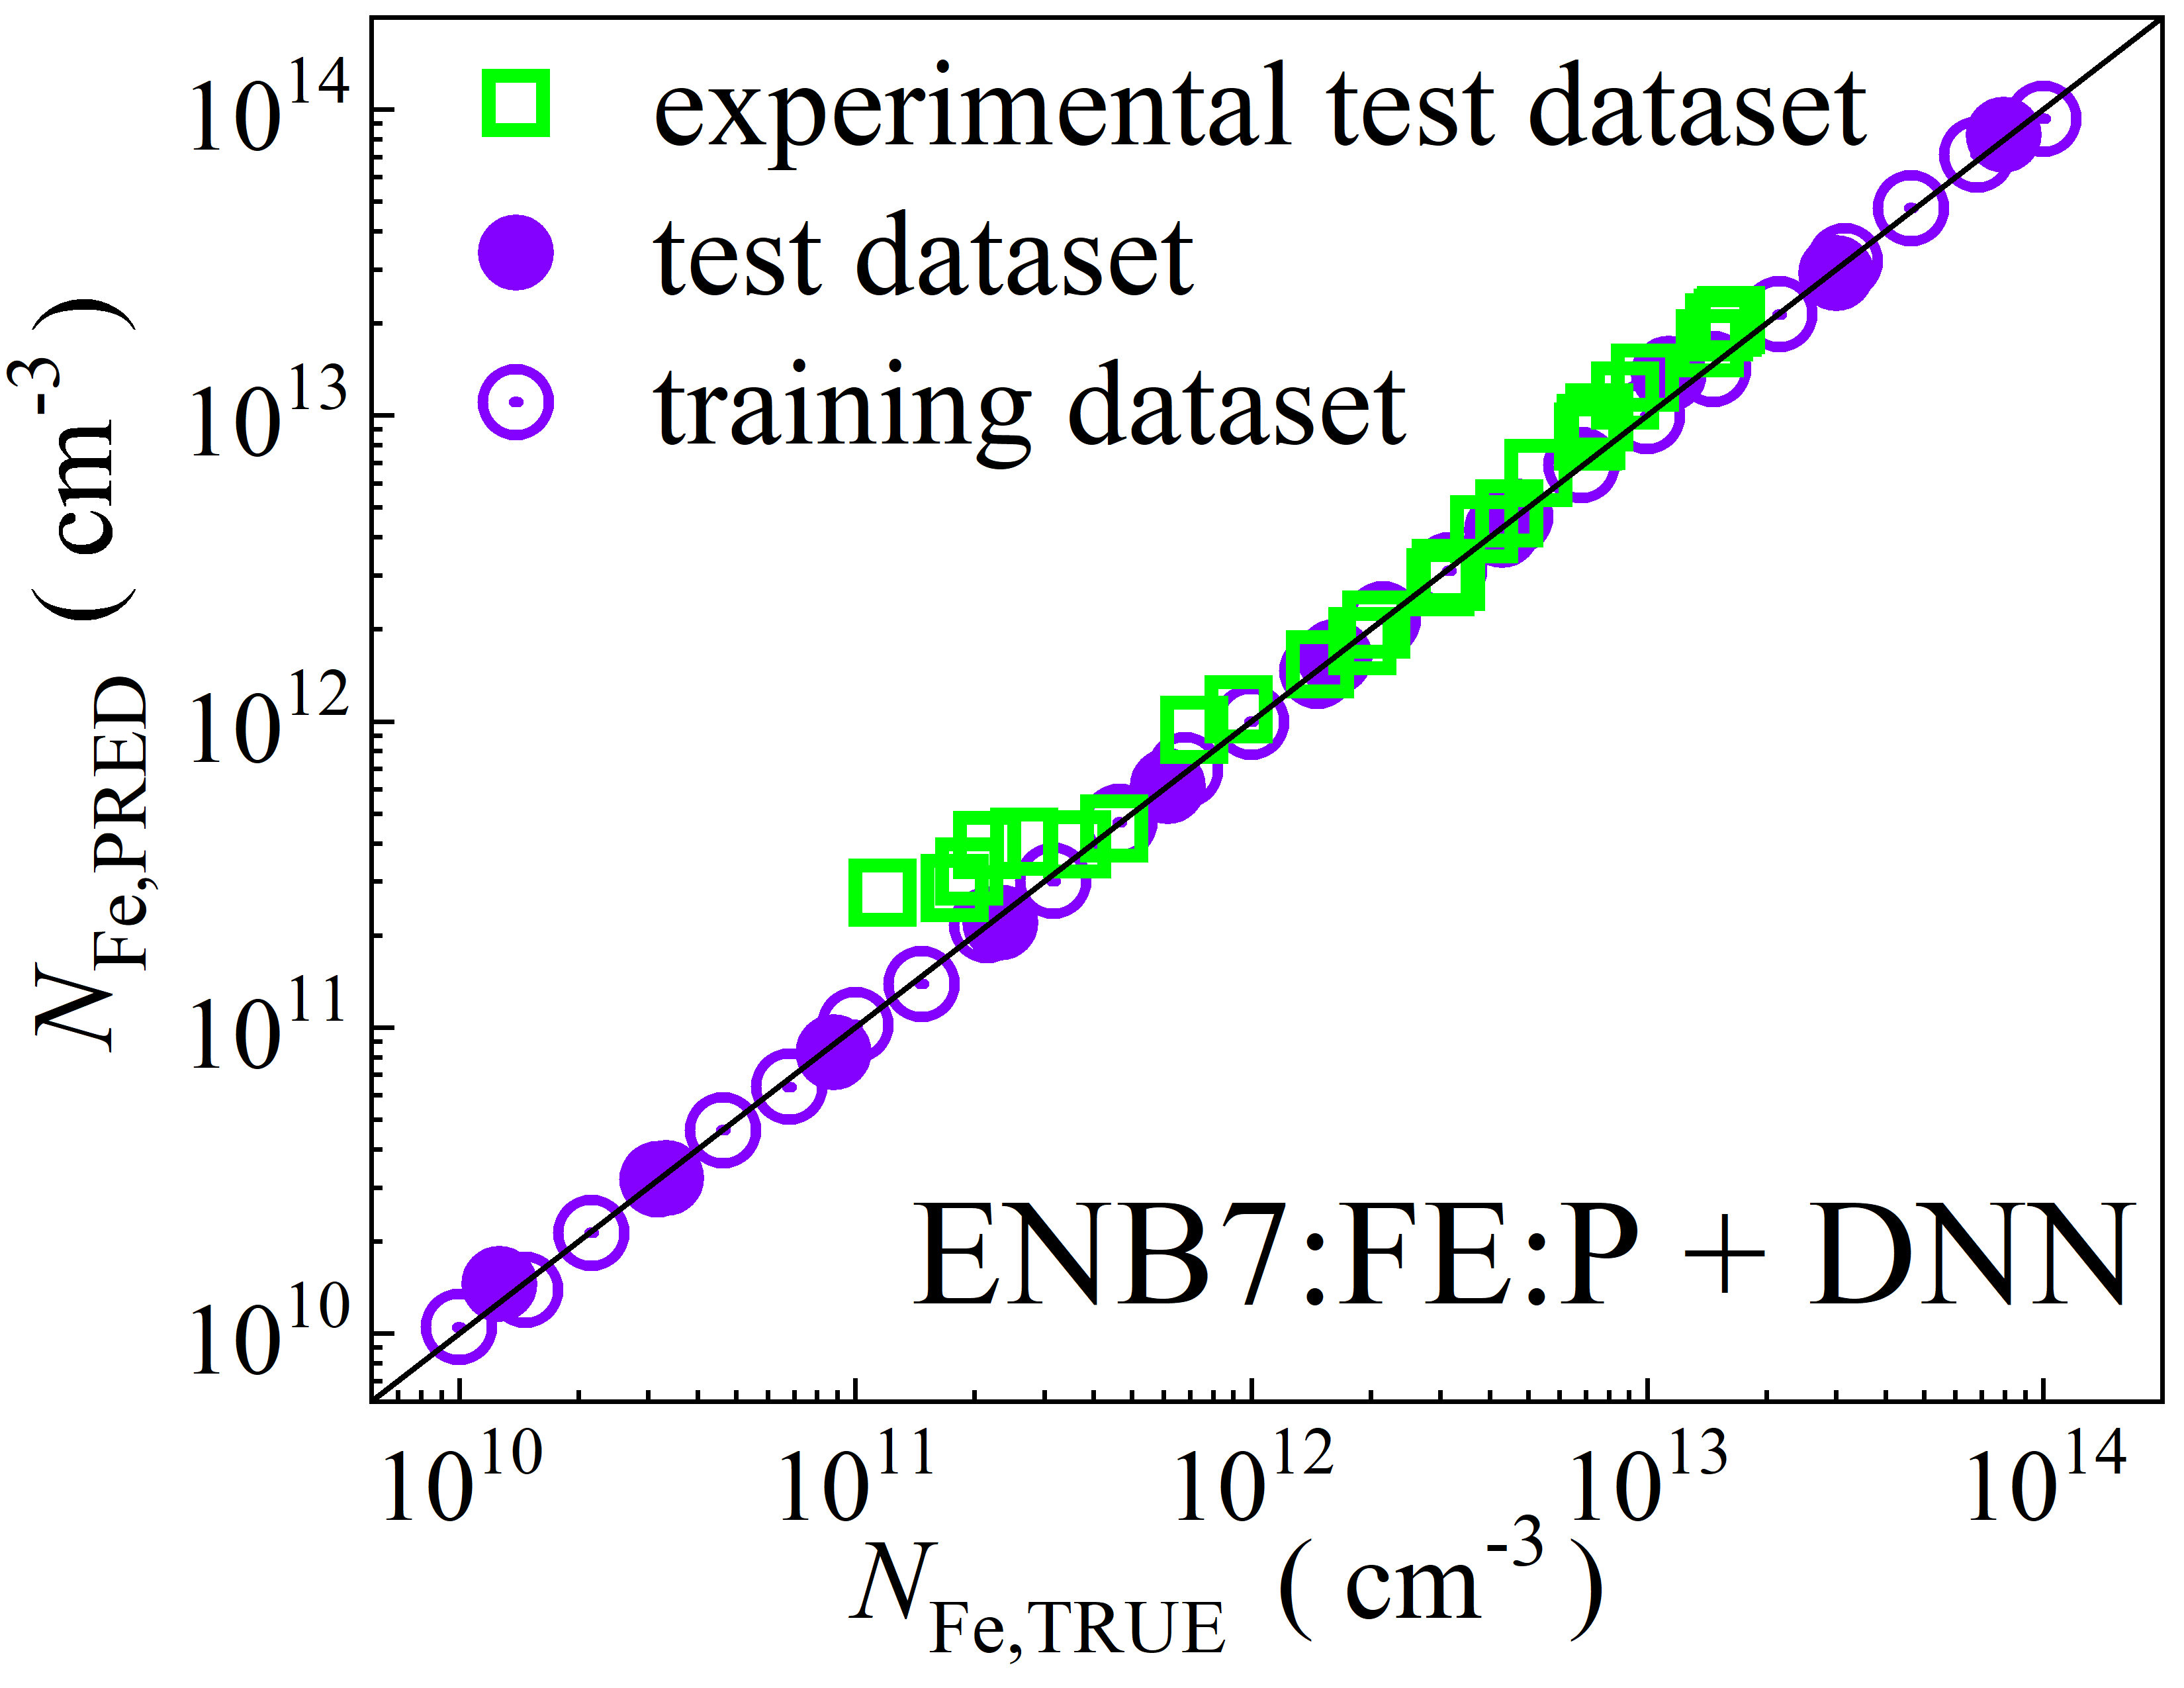
\includegraphics[width=0.4\linewidth]{Fig4a.png}
  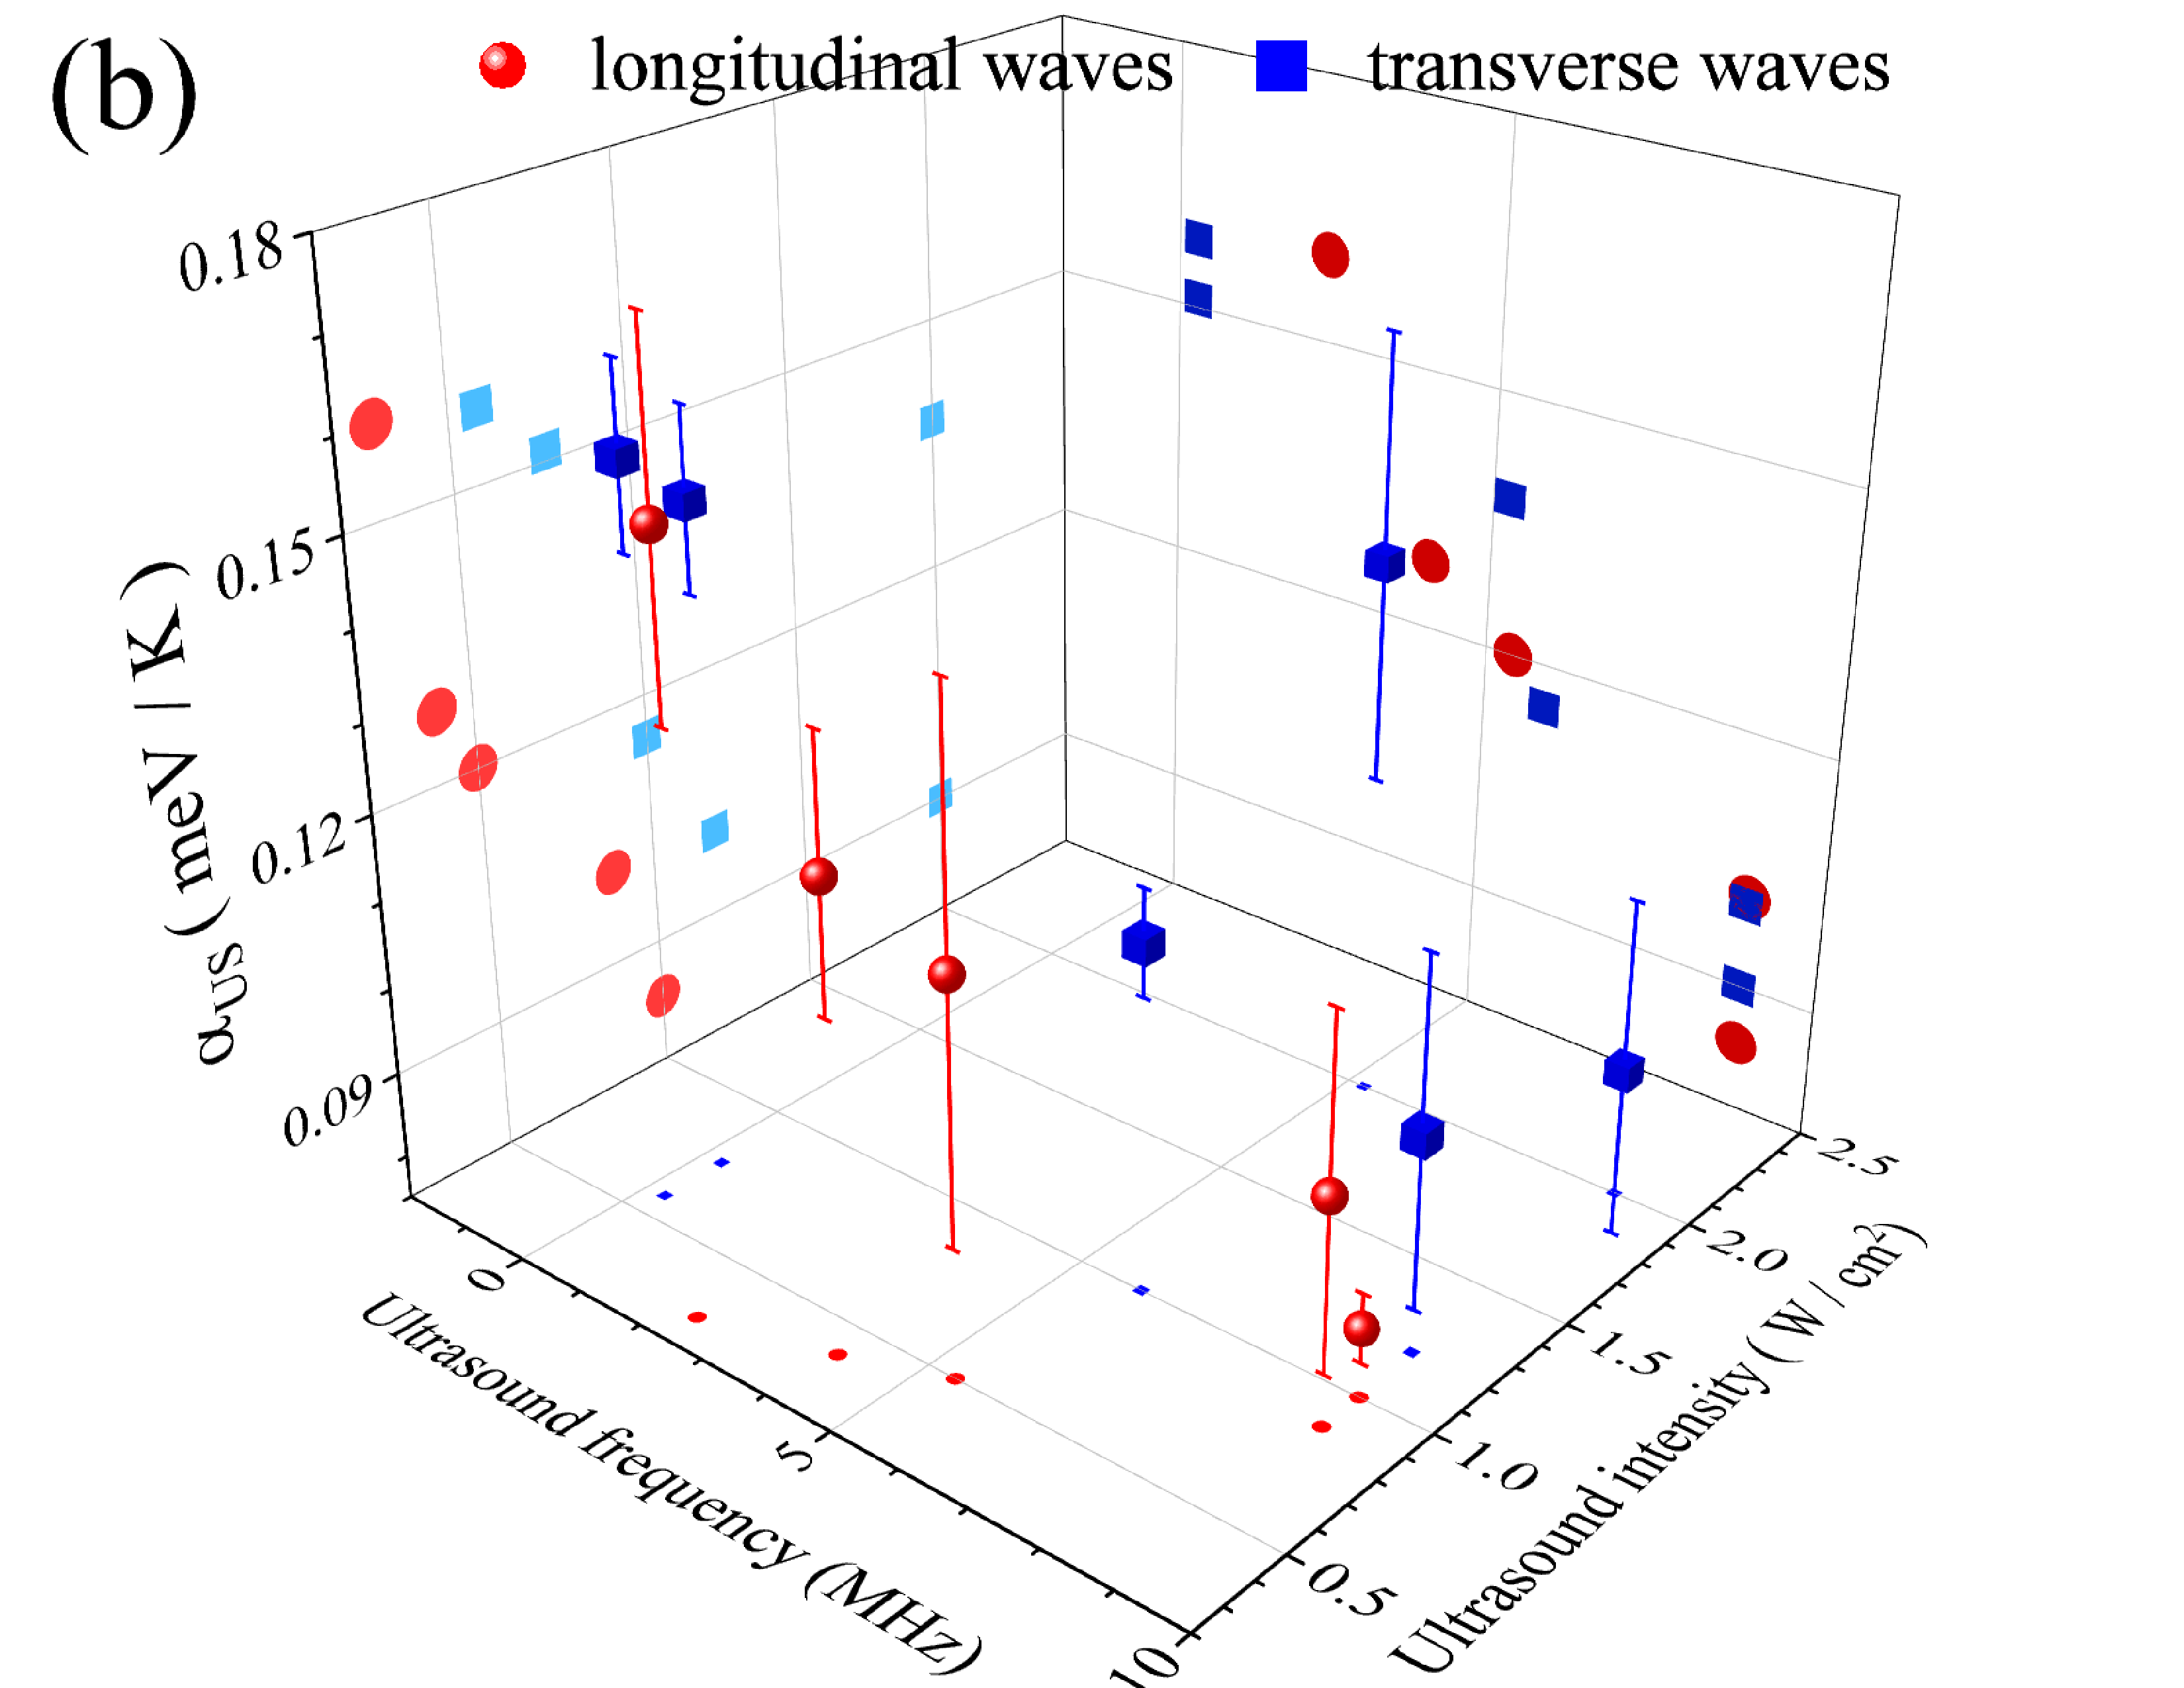
\includegraphics[width=0.4\linewidth]{Fig4b.png}
  \caption{
  The spectra of sample illumination in the case of using different light sources
  with the same integral intensity $W_\mathrm{ill}=400$~mW (panel a) and a single source (Osram)
 at various $W_\mathrm{ill}$ values (panel b).
 The inset shows photos of light sources.
}
  \label{fig4}
\end{figure}


Carrier generation rate was estimated as follows:
\begin{equation}
\label{eqGint}
G=\int g(\lambda) d\lambda\,,
\end{equation}
where spectral carrier generation rate $g$
\begin{equation}
\label{eqGspectr}
g=\frac{w_\mathrm{ill}\lambda}{hc}\frac{(1-R)A_\mathrm{bb}}{S\,d_\mathrm{eff}}\,,
\end{equation}
where $n_\mathrm{ph}=\frac{w_\mathrm{ill}\lambda}{hc}$ is the spectral photon flux,
$R$ is the is the reflectance,
$A_\mathrm{bb}$ is the fraction of the band-to-band transitions,
$S$ is the illuminated area of sample,
$d_\mathrm{eff}$ is the effective width of carrier generation.

In calculating the value of $R$, we employed an approach \cite{KostRefl2000},
which accounted for the presence of antireflective and passivating layers on the front surface of the sample,
as well as the effects of multiple reflections.
The resulting spectral dependence of $R$ is shown in Figure~S3 of the Supplementary materials.

The expression for the e-h pair generating fraction of the Lambertian absorptance in a solar cell
can be written as \cite{Schaefer2018}:
\begin{equation}
\label{eqAbb}
A_\mathrm{bb}(\lambda)=\frac{\alpha_\mathrm{bb}}{\alpha_\mathrm{bb}+\alpha_\mathrm{fca}}\frac{(1-T_r)(1+T_r)n_r^2}{n_r^2-(n_r^2-1)T_r^2}\,,
\end{equation}
with
\begin{eqnarray*}
T_r&=&(1-x)\exp(-x)+x^2E_1(x)\,,\\
x&=&(\alpha_\mathrm{bb}+\alpha_\mathrm{fca})d\,,\\
E_1(x)&=&\int_x^\infty t^{-1}\exp(-t)dt\,,
\end{eqnarray*}
where
$\alpha_\mathrm{bb}$ is the absorption coefficient due to e–h pair
generation by band-to-band transitions;
$\alpha_\mathrm{fca}$ is the absorption coefficient due to free carrier absorption;
$n_r$ is the refractive index;
$d$ is the width of the device.

In our calculations of $A_\mathrm{bb}$ by using Equations~(\ref{eqAbb}), we took  $\alpha_\mathrm{bb}$ and
$n_r$ from Green\cite{Green2022}, $\alpha_\mathrm{fca}$  from Baker-Finch \emph{et al.} \cite{SiFCA}.
The spectral dependence of the fraction of the band-to-band transitions can be found in Supplementary materials (Figure~S5).

When determining the carrier generation volume, we applied Bowden\&Sinton  approach \cite{Bowden2007} to thick silicon wafers,
where the diffusion length or light absorption depth is significantly less than the sample thickness.
In these cases, the distribution of carriers is heavily skewed toward the illuminated surface,
rendering the use of the arithmetic mean of carrier concentration unsuitable.
Consequently, the average values are computed using carrier concentration as a weighting function,
and effective generation region width is determined as follows \cite{Bowden2007}:

\begin{equation}
\label{eqdeff}
d_\mathrm{eff}(\lambda)=\frac{\left(\int_0^d \Delta n dx\right)^2}{\int_0^d \Delta n^2 dx}\,,
\end{equation}
where
$\Delta n$ is the increase in minority carrier density due to illumination
\begin{equation}
\label{eqdeln}
\Delta n (x)=\frac{\alpha_\mathrm{bb} n_\mathrm{ph} L_n^2 q}{(\alpha_\mathrm{bb}^2 L_n^2-1)kT\mu_n}
\left[\exp\left(-\frac{x}{L_n}\right)-\exp\left(-\alpha_\mathrm{bb} x\right)\right]\,.
\end{equation}
In calculations, we used $L_n$ value, determined in Section~\ref{SecR}.
Some dependencies for different $L_n$ values are shown in Figure~S4 (Supplementary materials).

The consideration of dependencies $R(\lambda)$, $A_\mathrm{bb}(\lambda)$, and $d_\mathrm{eff}(\lambda)$ alters
the spectral carrier generation rate compared to the spectral photon flux,
leading to an increased contribution to e-h pairs generating from shorter wavelength light,
as illustrated in \textbf{Figure~\ref{fig5}a}.
In \textbf{Figure~\ref{fig5}b}, variations in the total carrier generation rate are depicted with increasing light intensity for different light sources.
It is evident that differences exist between the light sources,
yet the absolute contrasts in the magnitude of $G$ for various light sources under $W_\mathrm{ill}=const$ conditions do not surpass 2 percent,
with Orion registering the highest carrier generation rate value.
Notably, without considering $R$, $A_\mathrm{bb}$, and $d_\mathrm{eff}$ and calculating $G$  as the ratio of incident photons number
to the total sample volume, the qualitative outcomes would remain quite similar. The main difference would lie in the absolute values of the carrier generation rate.

\begin{figure}
\centering
  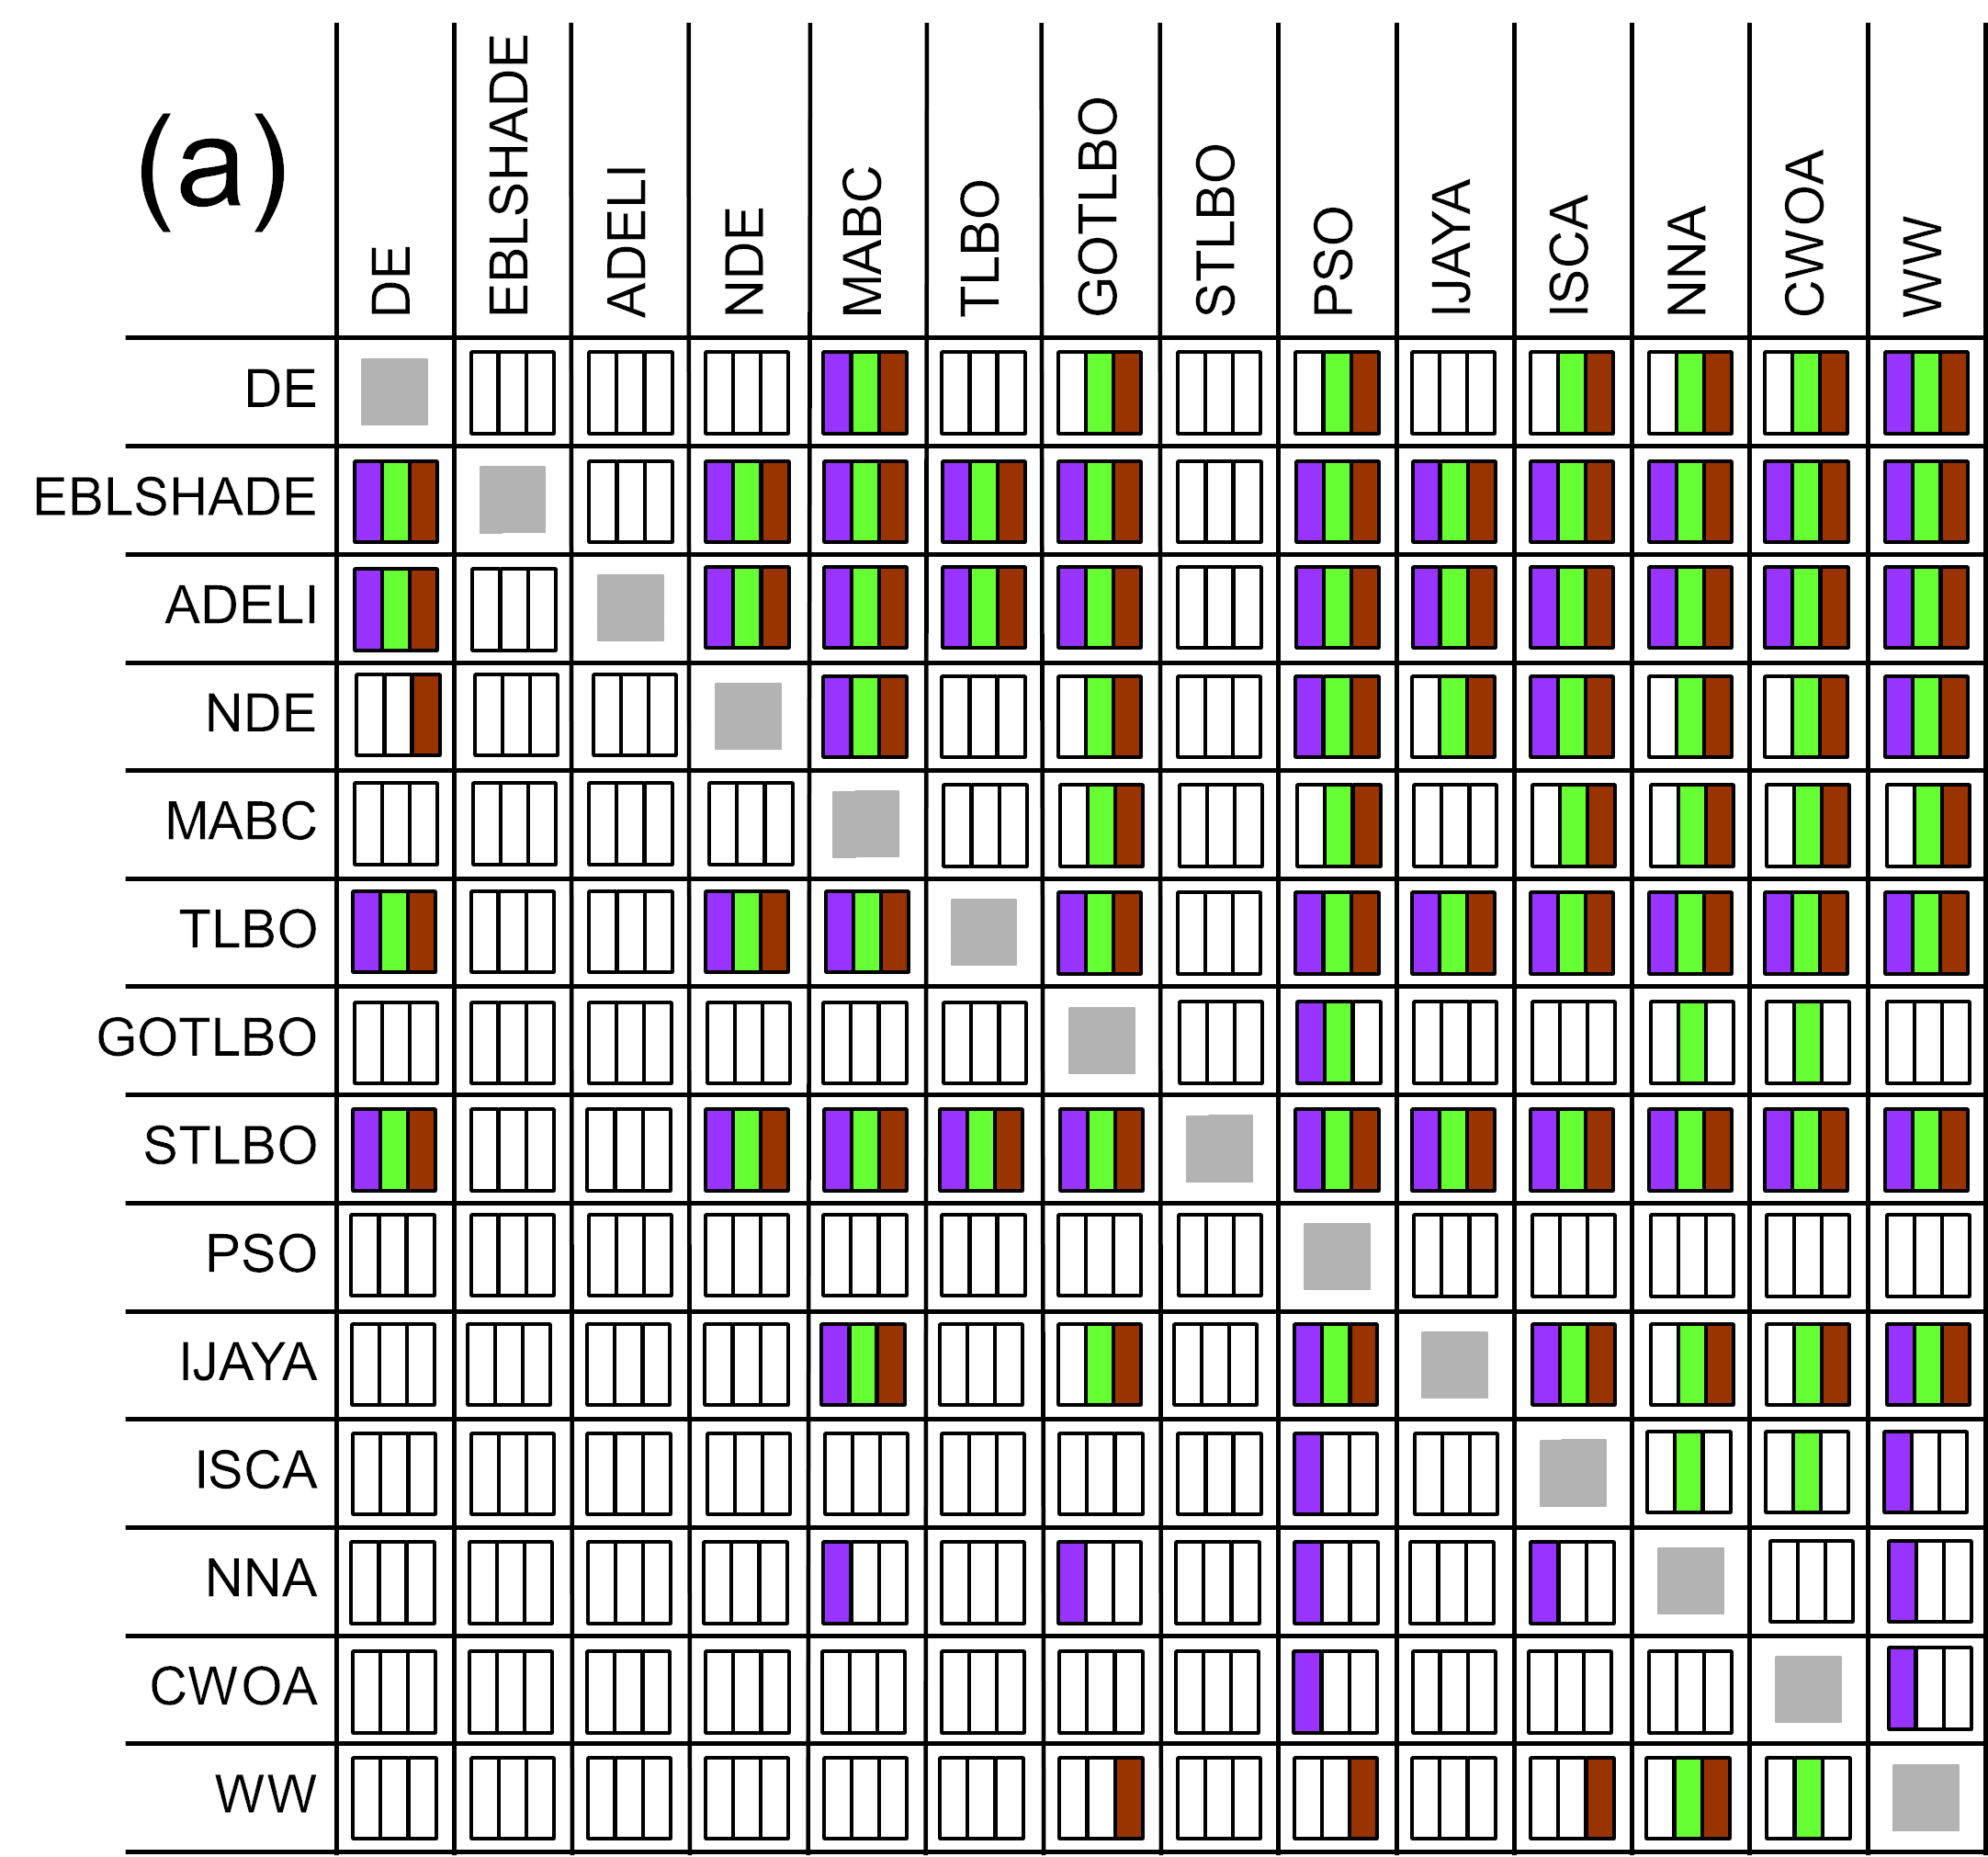
\includegraphics[width=0.4\linewidth]{Fig5a.png}
  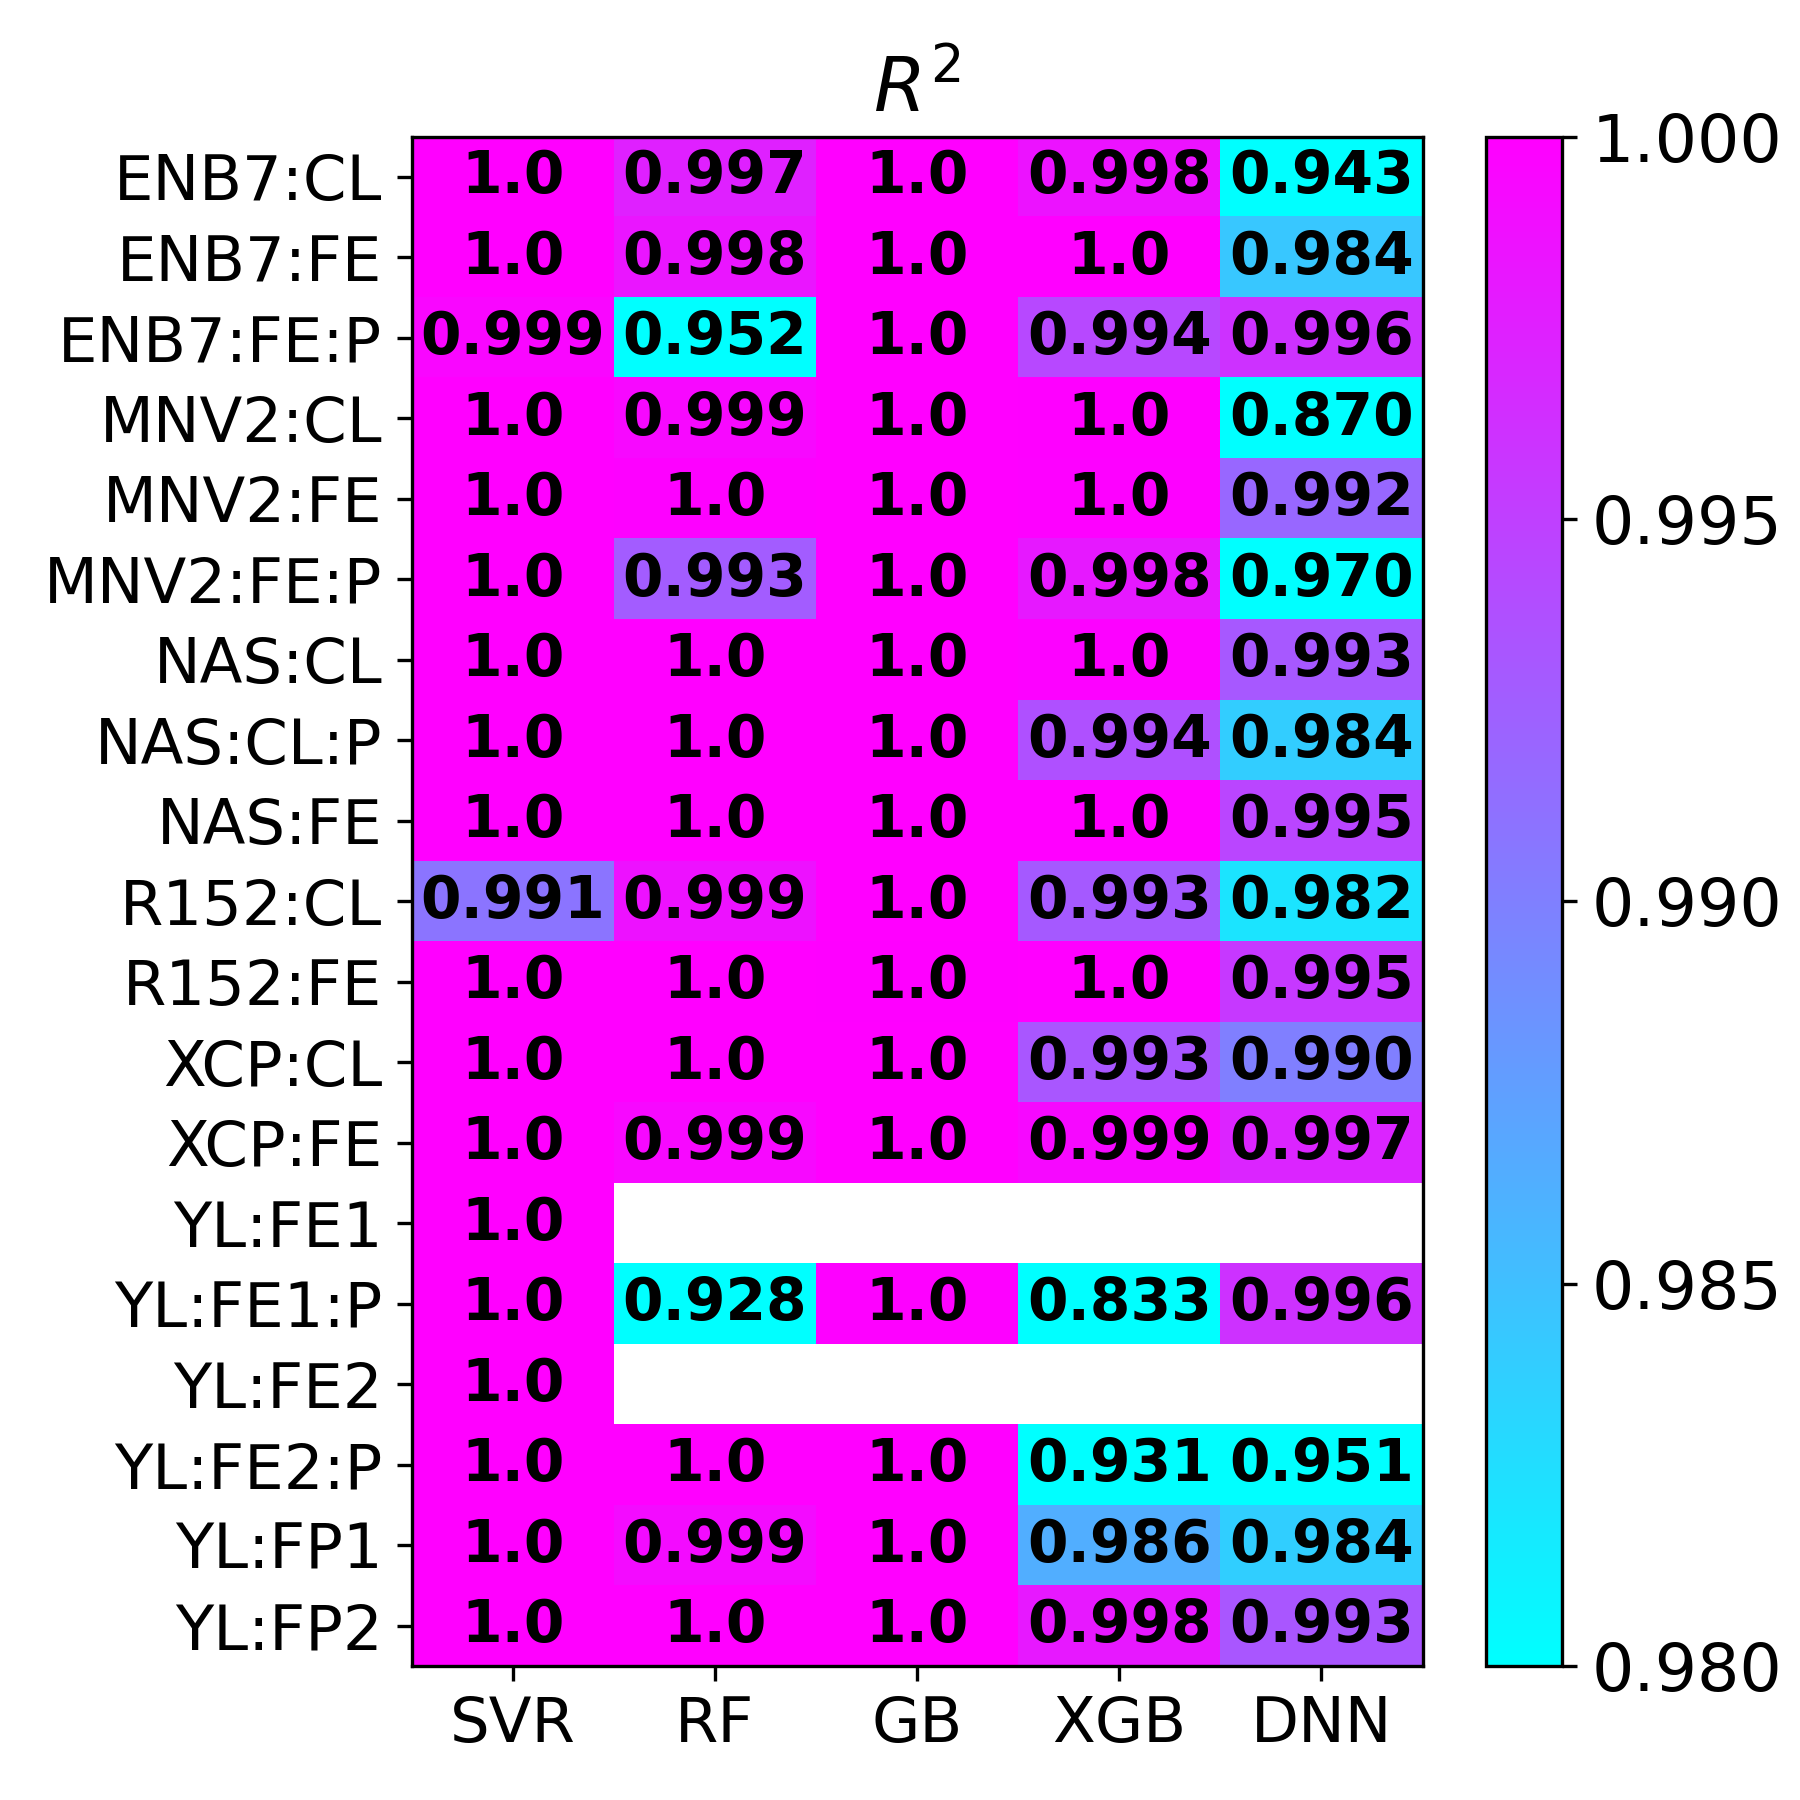
\includegraphics[width=0.4\linewidth]{Fig5b.png}
  \caption{
  (a) Photon flux spectral density (left axis, solid line) and carrier generate rate spectral density (right axis, dashed line).
  Orion light source, $W_\mathrm{ill}=400$~mW.
  (b) Dependencies of carrier generation rate on illumination intensity for different light sources.
  }
  \label{fig5}
\end{figure}

Thus, the discrepancies previously (Section~\ref{SecR}) noticed  in the value of $R_d$ under identical illumination intensity levels
cannot be attributed to variations in the carrier generation rate among different light sources,
even when factoring in the quadratic dependency of the dissociation rate on $G$.
Hence, there must be another underlying cause for these differences.


\subsection{Effect of illumination spectrum on FeB pair decay}\label{SecLast}

The dependencies $R_d (G)$ in logarithmic scale are presented in \textbf{Figure~\ref{fig6}a}.
The linear patterns observed in the data indicate a clear power law relationship between
the dissociation rates of FeB pairs and the carrier generation rate.
The figure also exhibits the fit results using Equation~(\ref{eqRd}).
High correlation coefficients exceeding 0.998 validate the applicability of the quadratic dependence expressed by Equation~(\ref{eqRd}) to our data.
It should be noted that Khelifati \emph{et al.} \cite{FeBKin2019} stipulate the inclusion of
$R_d\left(1+\tau_\mathrm{FeB}/\tau_\mathrm{other}\right)^2$ (where $\tau_\mathrm{FeB}$ is the lifetime associated with recombination on FeB pairs)
on the left-hand side of Equation~(\ref{eqRd}) rather than $R_d$.
However, in our cases $\tau_\mathrm{other}\gg \tau_\mathrm{FeB}$, as previously acknowledged in Section~\ref{SecR},
this additional multiplier can be disregarded.


\begin{figure}
\centering
  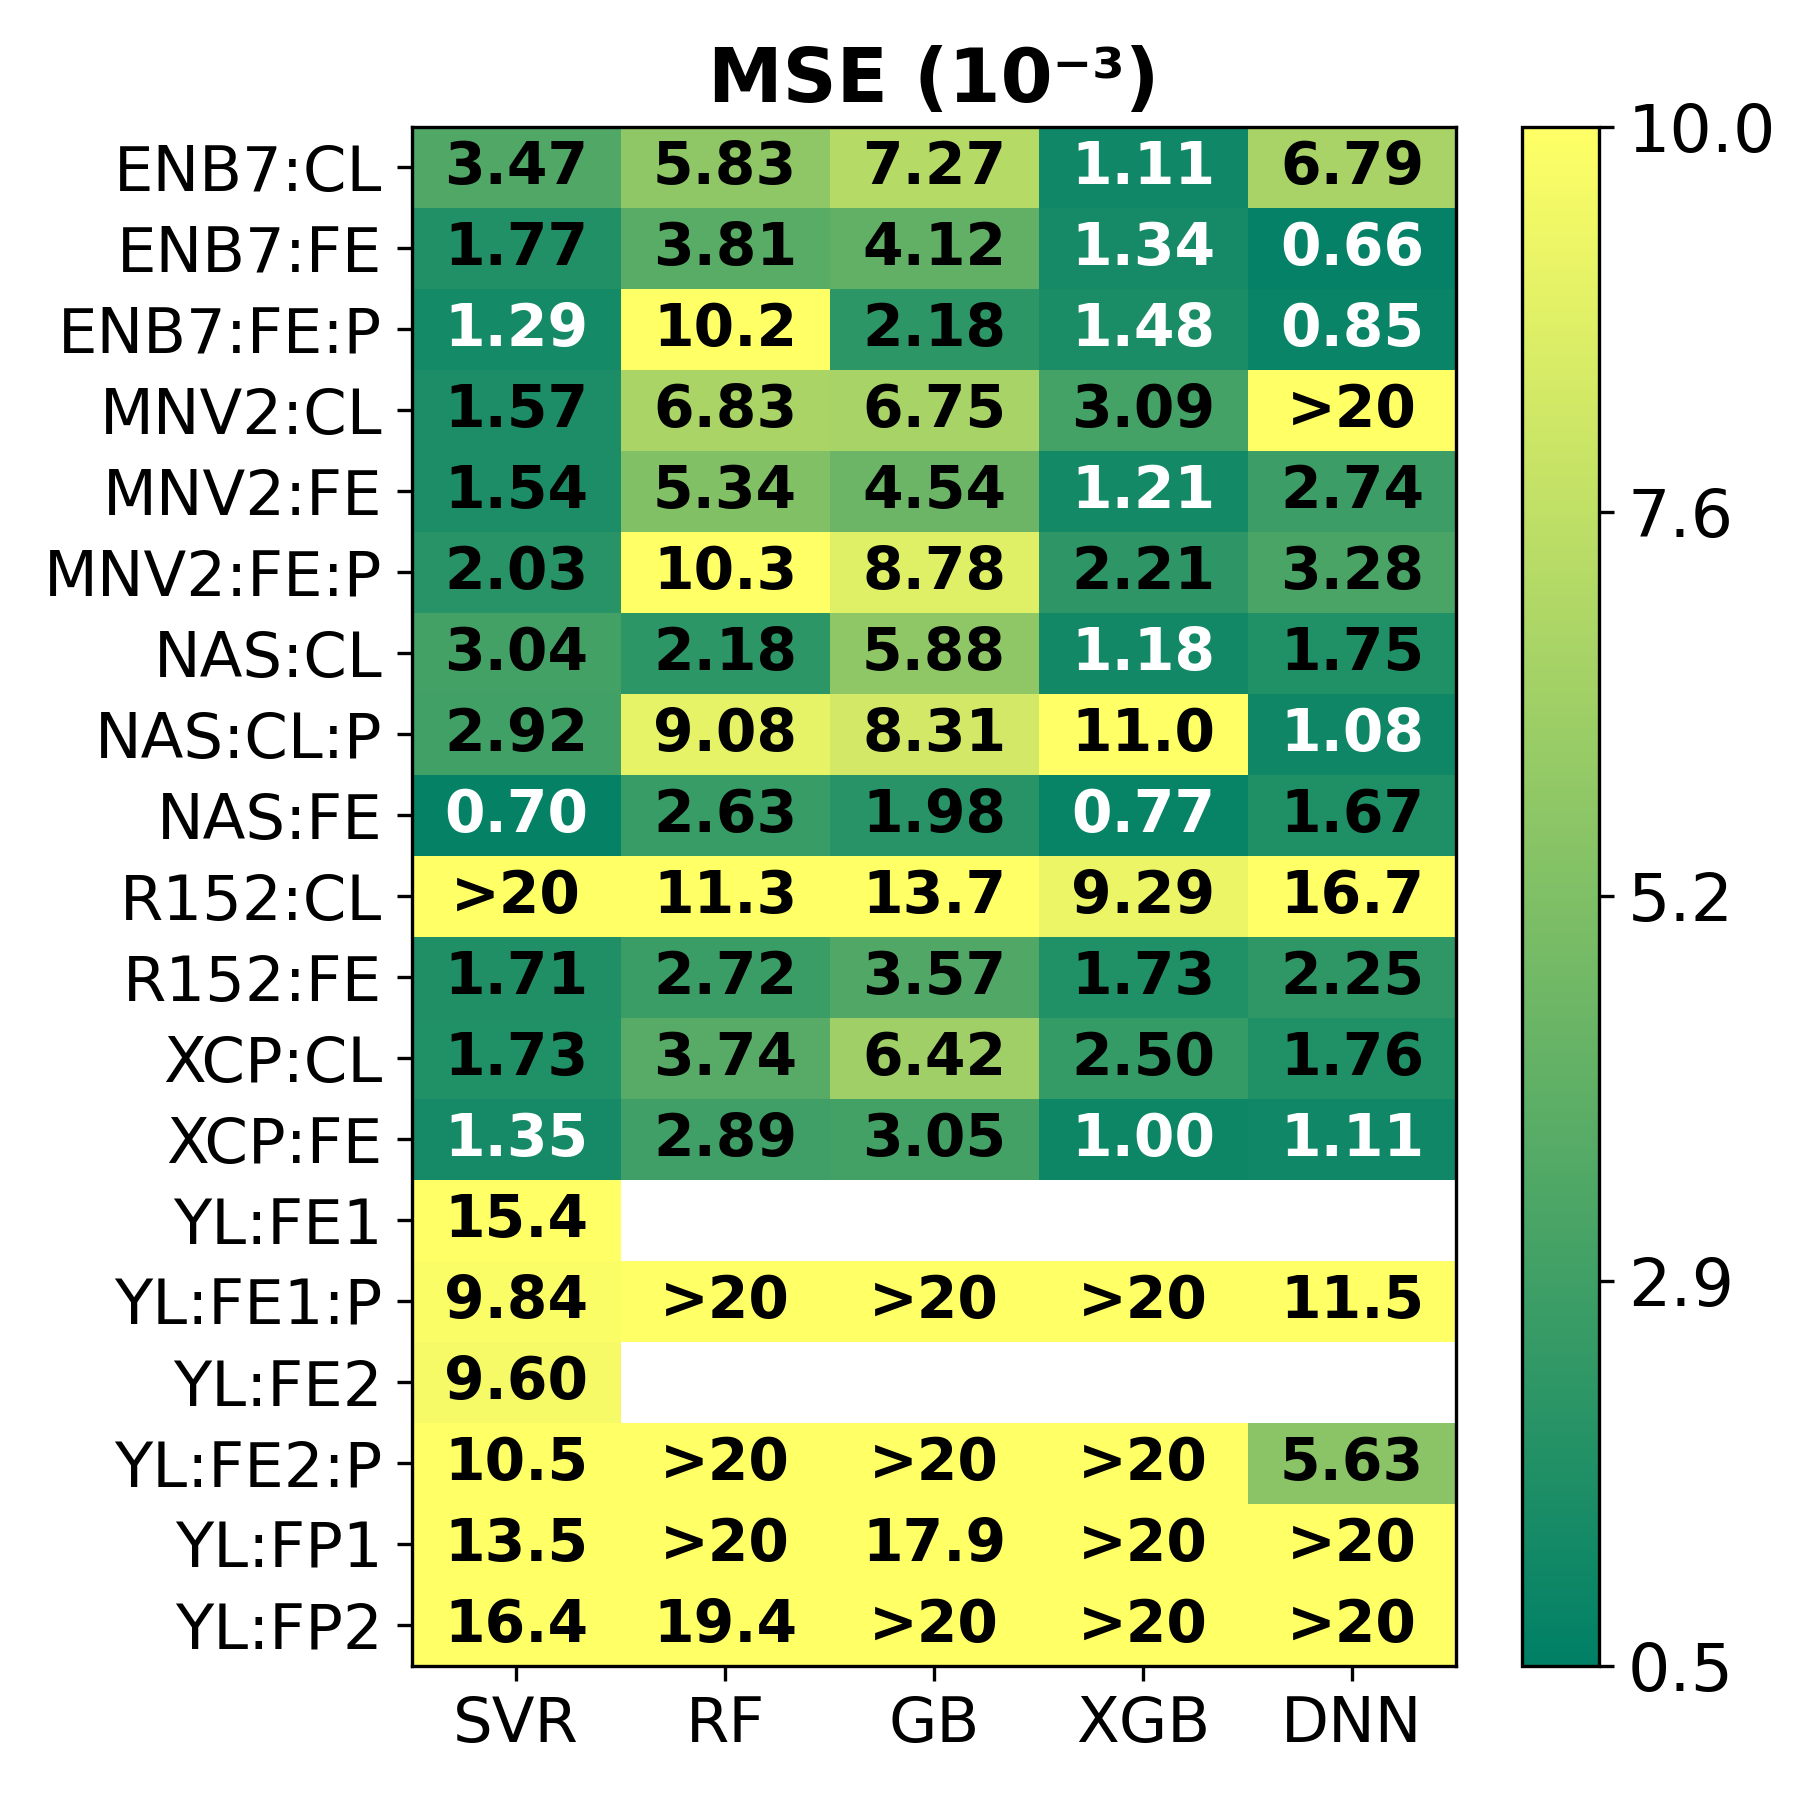
\includegraphics[width=0.4\linewidth]{Fig6a.png}
  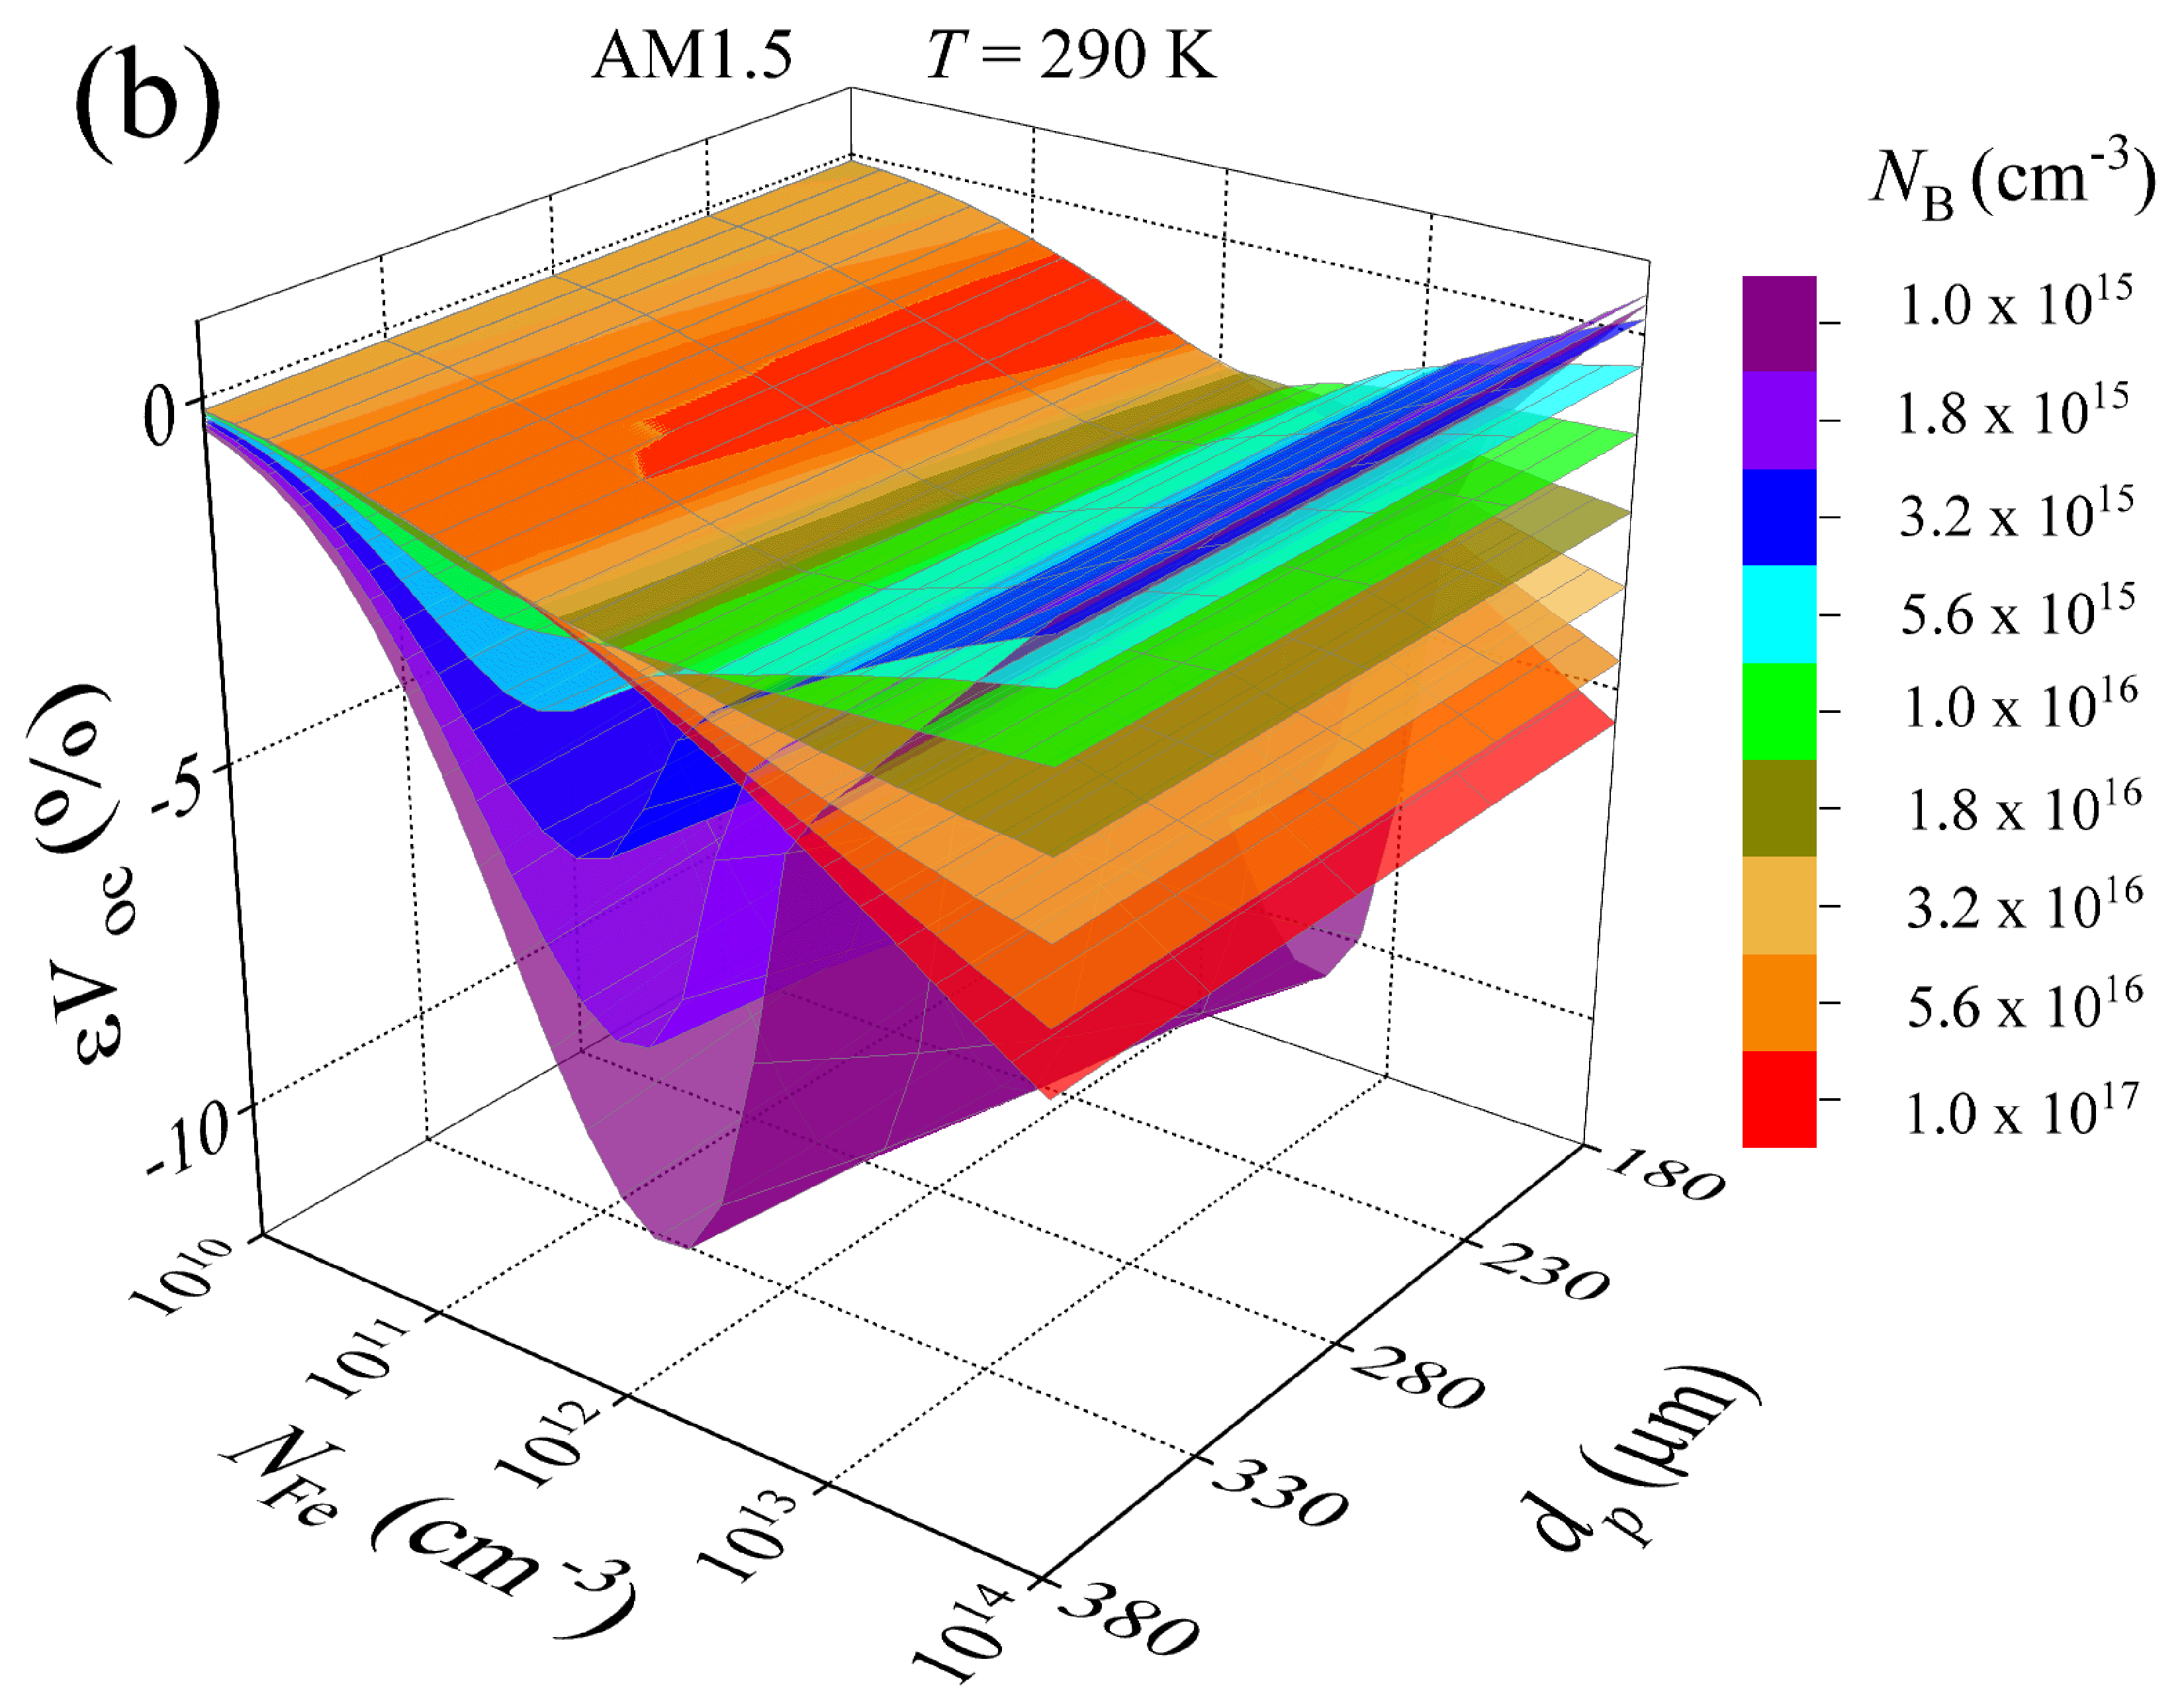
\includegraphics[width=0.4\linewidth]{Fig6b.png}
  \caption{
  (a) FeB pair dissociation rate plotted as $R_d\cdot N_\mathrm{FeB}^2$ over the light induced
  generation rate. The solid lines show the quadratic dependence according to Equation~(\ref{eqRd}).
  (b) Dependencies of average photon energy on illumination intensity for different light sources.
  The inset shows prefactor $K$ vs average photon energy for the different light sources and illumination intensities.
  The lines are linear fitting curves. Coefficients of correlation are shown as well.
  }
  \label{fig6}
\end{figure}

The prefactor $K$ values determined from the fitting are
$3.8\times10^{-15}$~s for the GE light source,
$2.0\times10^{-15}$~s for the Osram, and
$1.5\times10^{-15}$~s for the Orion source.
$K$ serves as a important parameter linked to the phenomenon of FeB pairs' dissociation by illumination \cite{FeBKin2019},
and the values obtained in this study are compared with those ($4.2\times10^{-17}-5\times10^{-15}$~s) previously presented \cite{FeBLight2,FeBAssJAP2014,FeBKin2019}.
It is essential to note that in prior research, disparities in the constant $K$ value for diverse samples were ascribed
to variations in defect composition and the presence of alternative recombination channels apart from iron-related defects \cite{FeBLight2,FeBAssJAP2014}.
Early, the dependence of $R_d$ on temperature was reported as well \cite{Lagowskii1993}.
However, in our case, distinct $K$ values were obtained for the same structure under identical conditions, such as temperature and integrated light intensity,
with differences in the illumination spectra only.

In other words, the obtained data indicate that in the analysis of light-induced dissociation of FeB pairs,
it is necessary to consider not only the quantity of photo-generated excess charge carriers
but also the energies of the photons that lead to their appearance.
For such an energy characterization of light sources, we used the average photon energy $<E_\mathrm{ph}>$:
\begin{equation}
\label{eqEaver}
<E_\mathrm{ph}>=\frac{\int \frac{hc}{\lambda}n_\mathrm{ph}(\lambda)d\lambda}{\int n_\mathrm{ph}(\lambda)d\lambda}\,.
\end{equation}


The summary of the results concerning the $<E_\mathrm{ph}>$ values is shown in \textbf{Figure~\ref{fig6}b}.
In particular, it demonstrates the shift of the emission spectrum of light sources
towards the short-wavelength region with an increase in the $W_\mathrm{ill}$ value, as illustrated in Figure~\ref{fig4}a.
And a clear conclusion can be drawn upon comparing the data in Figure~\ref{fig3},\ref{fig5}b, \ref{fig6}a, \ref{fig6}b
and Table~\ref{tb1}:
with rising average photon energy, the light-induced dissociation of FeB pairs becomes more pronounced.
Specifically, the constant $K$ increases, the dissociation rate $R_d$ escalates,
and correspondingly, the illumination time necessary for a complete complex decay decreases.
Consequently, for the dissociation of FeB pairs, the energy expended during the thermalization of non-equilibrium carriers also holds significance.

The obtained results offer some conclusions about the mechanism of FeB dissociation.
As discussed in the literature and previously mentioned, two possible ways of the second decay stage
are typically considered: REDR and the recharge of the iron ion.
REDR arises from strong electron-lattice coupling at the defect site
and involves the utilization of local vibrational energy to promote pair dissociation \cite{FeBAssJAP2014,Sun2021,Macdonald2004}.
The observed correlation between dissociation rate and photon energy in this study supports the REDR process.
Specifically, as photon energy increases, the production of non-equilibrium phonons during thermalization also rises.
Furthermore, the increase in $R_d$ value, as found in the experiment, signifies the active involvement of these quasi-particles in the dissociation of FeB pairs.
Notably, recent research \cite{Sun2021} focusing on a detailed analysis of the dissociation and association reactions of the iron-boron pairs similarly concluded the predominant role of REDR processes.



\section{Conclusion}\label{SecConsl}

The effect of the illumination spectra on the dissociation of
FeB pairs in p-Si was investigated in this paper.
We reported the results of a experimental systematic study on FeB dissociation rate in solar cell based on Cz-Si,
which were carried out using different light source and illumination intensities.

The findings showed that the time required for a total dissociation of the FeB pairs
not only becomes shorter with the increase of illumination intensity but also significantly depends
on light source.
As a result, the value of material constant $K$  varies and has been determined to be
$3.8\times10^{-15}$~s, $2.0\times10^{-15}$~s, and $1.5\times10^{-15}$~s
for three different light sources.
The study of the illumination spectrum led to the conclusion that the
efficiency of FeB photo-dissociation increases with a decrease in light wavelength.
The observation of an increase in the dissociation rate
with photon energy indicates that
the REDR effect prevails as the dominant factor during the second stage of light-induced dissociation of FeB pairs.
Furthermore, the obtained results could help to develop defect engineering procedures
for effectively converting iron impurities in silicon into high-mobility states,
which could significantly impact semiconductor technology.


% Experimental section

\section{Experimental Section}
\label{SecExp}

The $n^+$-$p$-$p^+$-Si samples were used in the experiment.
The structure was fabricated from a 380~$\mu$m thick $p$-type boron-doped
Czochralski silicon (100) wafer with hole concentration $p=1.36\times10^{15}$~cm$^{-3}$.
The $n^+$ emitter with sheet resistance of about $20-30$~$\Omega/\Box$
and  thickness of $0.7$~$\mu$m was formed by phosphorus diffusion.
The anti-recombination isotype barrier was created by using a $p^+$
layer ($10-20$~$\Omega/\Box$, $0.6$~$\mu$m) formed by boron diffusion.
On the front surface, the antireflective and passivating SiO$_2$ (40~nm) and Si$_3$N$_4$ (30~nm) layers
were formed.
The solid and grid Al contacts were formed by magnetron sputtering on the rear and front surfaces respectively.

Three powerful halogen lamps from different manufacturers were used for sample illumination and were employed for the light-induced dissociation of FeB pairs:
\begin{itemize}
  \item Orion Haltlichtspiegel 52240.0, 24 V, 200 W (labeled Orion in the paper);
  \item Osram 64653 HLX ELC, 24 V, 250 W (Osram);
  \item General Electric 43537 H271, 20 V, 150 W (GE);
\end{itemize}
The light sources were powered by the DC Power Supply ITECH IT6332B, which allowed setting the current passing through the lamp with an accuracy of up to 1 mA.

The illumination originating from the sources was transmitted to the sample via fiber.
The sources' emission underwent calibration at the fiber output,
thereby enabling a direct assessment of the light flux incident on the sample.
The relationships between the integral illumination intensity
and the current consumed by the sources were measured using an optical power and energy meter Thorlabs PM100D and a high-resolution sensor S401C.
The illumination spectra measurements were performed using spectrometer IKC-6 with germanium photodiode.
When analyzing the spectra, the spectral sensitivity of the photodiode was considered.

The current-voltage characteristics were measured using a Keithley 2450 source meter and
low--intensity monochromatic light source (light--emitting diode SN--HPIR940nm--1W with light wavelength 940~nm and intensity of about 400~$\mu$W).
The LED radiation intensity was stabilized by utilizing the W1209 thermostat and a power supply regulated by a circuit incorporating positive feedback and digital control.

The measurements were carried out at a temperature of 340~K.
The sample temperature was driven by a thermoelectric cooler,
controlled by an STS-21 sensor,
and maintained constant through a PID algorithm embedded in the software that serves the experimental setup.


%Frequency dependent capacitance-voltage (C–V-f) and conductancevoltage (G-V-f) measurements have been performed using a HP 4194 A Impedance Analyzer.
%The current-voltage (I–V) characteristics have been measured with the experimental setup shown in Fig. 3.
%The setup contains a GPIB connection to enable data transfer and acquisition between a Keithley Model 2400 Source Meter Unit (SMU) and a computer.

%All capacitance-voltage and photodiode measurements were performed inside a Vötsch VCL 4006 climatic chamber
%after a 15 min waiting period to let the samples adapt to the set temperature.
%For C − V measurements an Agilent E4990 A LCR meter was used.
%An RMS value of 30 mV was set during all measurements to maintain the linearity of the response and to stay below the current limit of the LCR meter.
%The device irradiance was measured with a Thorlabs FDS10x10 photodiode.
%The LED was driven and measured by a Keithley 2602 A.
%The EL spectra of the LEDs were measured using a Thorlabs IS200-4 Integrating sphere
%and an AvaSpec-ULS2048x64TEC spectrometer from Avantes.
%The spectrometer was calibrated in the wavelength range of 350 nm to 1100 nm with an Avalight-HAL-CAL mini lamp from Avantes.
%All measurements were controlled with a Matlab program.
%
%Current-density–voltage (J–V) and Suns–Voc measurements were performed in-house using an FCT-450 tool from Sinton instruments at
%standard test conditions.
%Impedance spectroscopy (IS) and the capacitance–voltage (C–V) measurements were performed at room temperature using
%a computer-controlled Keysight B1500A Semiconductor Device Analyzer with B1520A multi-frequency capacitance measurement unit (MFCMU).
%The impedance was measured as a function of frequency from 1 kHz to 1 MHz, with an AC perturbation signal of 10 mV.
%The measured impedance was fitted using the EIS Spectrum Analyzer software.

%J-V curves were measured using a Keithley 2400 Sourcemeter and a Steuernagel SolarCellTest 575 sun-simulator.
%Impedance spectra were measured using an IM6 Electrochemical Workstation from Zahner-elektrik.
%Samples were measured inside a flow cell, where a constant nitrogen flow was set in order to avoid degradation.
%A halogen lamp was used for illumination.
%Impedance spectra were recorded by applying a small voltage perturbation (20 mV rms) at frequencies from 1 MHz to 1 Hz in dark
%conditions (for voltages varying from 3 to 1 V).
%Illumination measurements were performed varying the irradiation intensity up to one sun (i.e., simulated AM 1.5 G, 1000 W/m2), under open circuit conditions.
%
%The J-V measurements are performed in a N2-filled glovebox under AM1.5G 100 mW=cm2 illumination from
%a class AAA solar simulator (Abet Technologies) using a low-noise sourcemeter (2635 A, Keithley) controlled by a LabVIEW program.
%The solar simulator intensity is set using a National Institute of Standards and Technology-traceable calibrated photodiode (Abet RR_227KG5).
%A 2.5-mmdiameter aperture is placed in front of each device to rigorously define the illumination area of 0.049 cm2.
%Impedance spectroscopy (IS) measurements used for extracting the capacitance value are carried out in an O-ring sealed sample holder containing N2 at room temperature
%using a Zahner IM6 electrochemical workstation.
%They are performed in the dark with an ac bias (20 mV) modulating between 1 Hz and 1 MHz.

%Device Characterization.
%The current density-voltage-luminance characteristics were measured using a Keithley 2450 source meter and
%a Konica Minolta luminance meter LS-150.
%The electroluminescence spectra were collected using a Topcon SR-UL2 Spectroradiometer.
%The photoluminescence spectra were obtained using a fluorescence spectrometer (Edinburgh, FLS 920).
%The capacitance spectra were recorded using an impedance analyzer (Keysight, E4990A).
%The optical permittivity was measured using a dual rotating-compensator Mueller matrix ellipsometer (Wuhan Eoptics Technology Co., ME-L ellipsometer).
%The low temperature environment in the experiments was provided by a cryostat system (Janis, ST-100).
%
%The temperature was maintained constant using a PID (proportional-integral-derivative controller) algorithm which is implemented in the software which serves the system.
%
%Therefore, the temperature of the
%wafers was regulated and controlled through a thermoelectric
%cooling system based on the Peltier effect

%\threesubsection{First part of experimental section}\\
%\threesubsection{Second part of experimental section}\\



\medskip
\textbf{Supporting Information} \par %Please delete the Suppporting Information statement if it is not applicable. Please supply Supporting Information in another file. Supporting information should not be provided in .tex format
Supporting Information is available from the Wiley Online Library or from the author.



% Acknowledgements
\medskip
\textbf{Acknowledgements} \par %delete if not applicable))
The authors are grateful for the help with calculating the reflectance by solar cells to Prof.~Vitaliy Kostylyov.

\medskip
\textbf{Conflict of Interest}\par
The authors declare no conflict of interest.

\medskip
\textbf{Data Availability Statement}\par
The data that support the findings of this study are available from the corresponding author upon reasonable request.
% References
\medskip


\bibliographystyle{MSP}
\bibliography{olikh}

%покращ англійську мову, використавши стиль наукової статті, та виправ граматичні і стилістичні помилки


% Figures/tables and captions
% Permission statements are required for all figures reproduced or adapted from previously published articles/sources. Please also ensure that all necessary permissions to reproduce images have been received
% Please remove these statements for original figures


%\begin{figure}
%  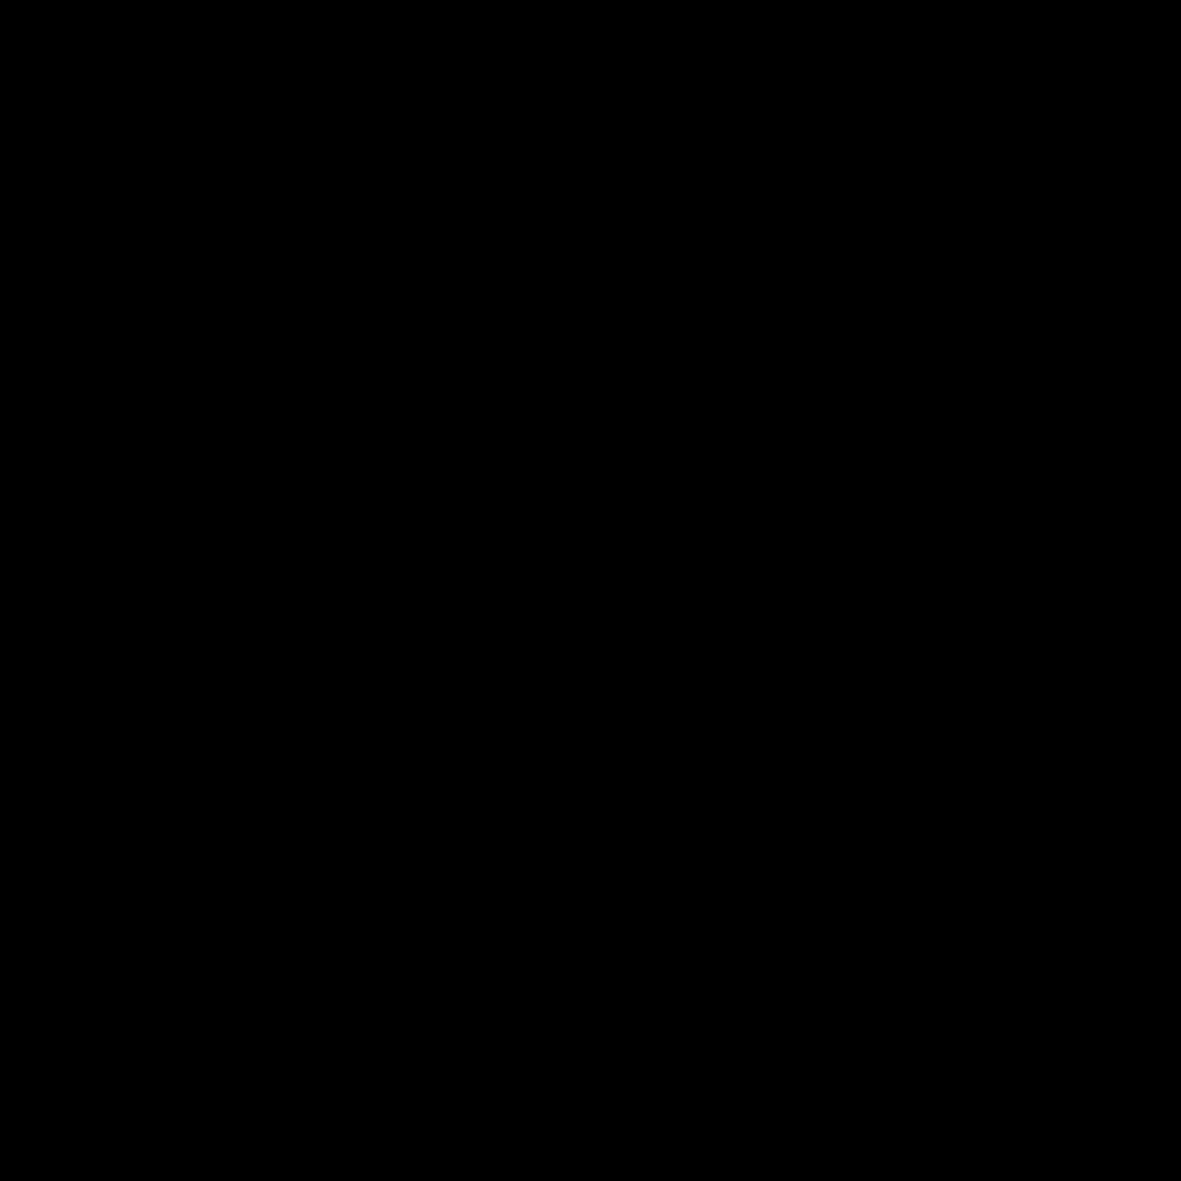
\includegraphics[width=\linewidth]{placeholder-image.png}
%  \caption{Figure 1 caption goes here. Reproduced with permission.\textsuperscript{[Ref.]} Copyright Year, Publisher. }
%  \label{fig:boat1}
%\end{figure}
%
%\begin{figure}
%  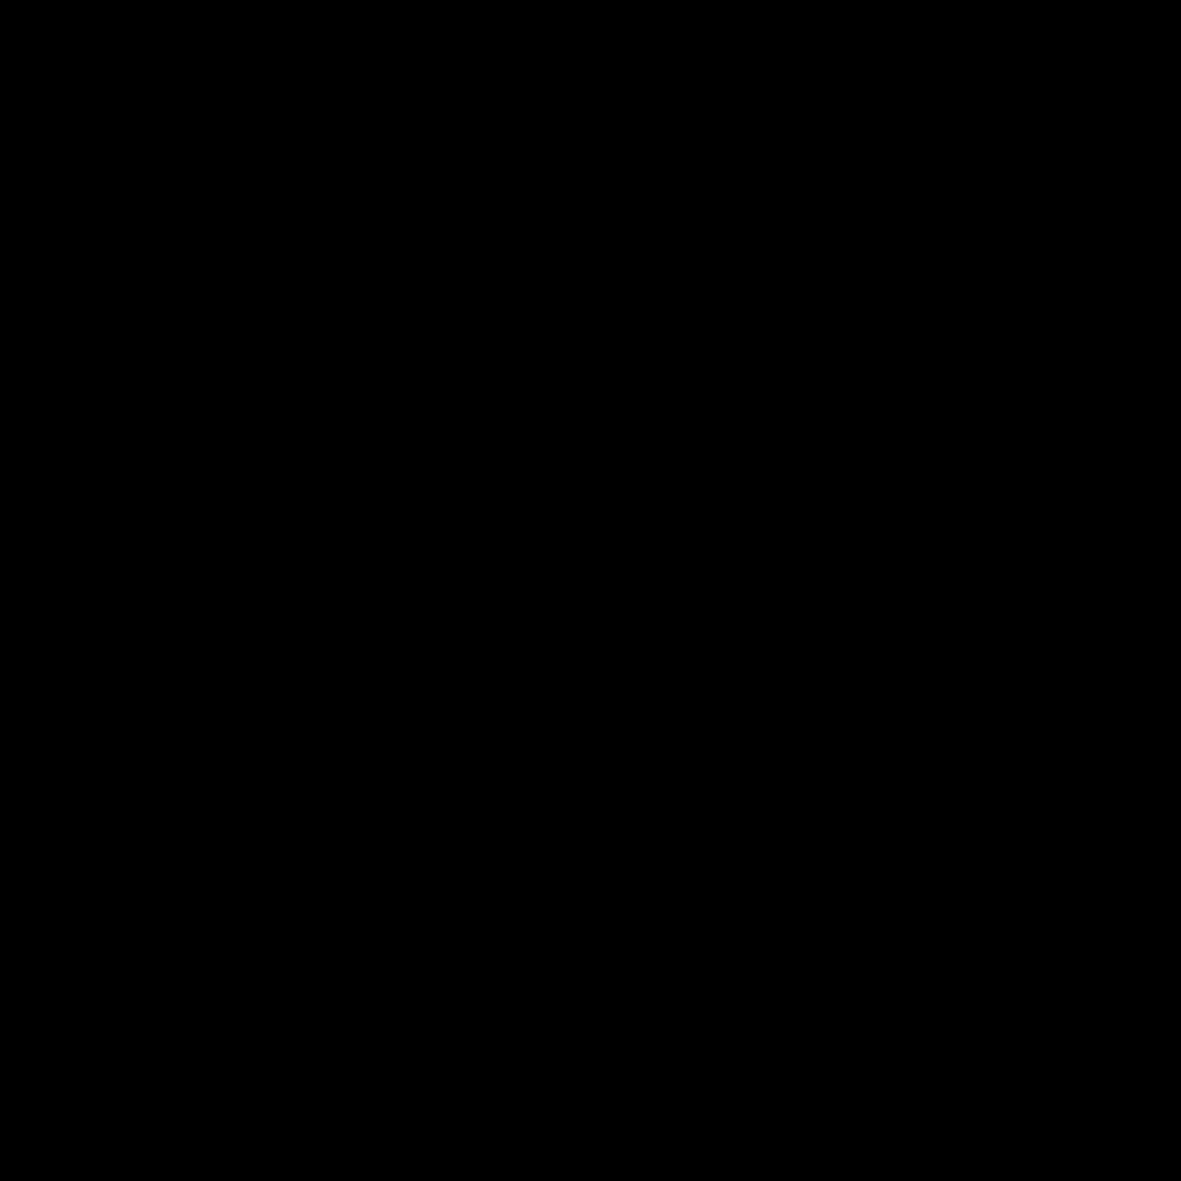
\includegraphics[width=\linewidth]{placeholder-image.png}
%  \caption{Figure 2 caption goes here. Reproduced with permission.\textsuperscript{[Ref.]} Copyright Year, Publisher.}
%  \label{fig:boat1}
%\end{figure}
%
%\begin{figure}
%  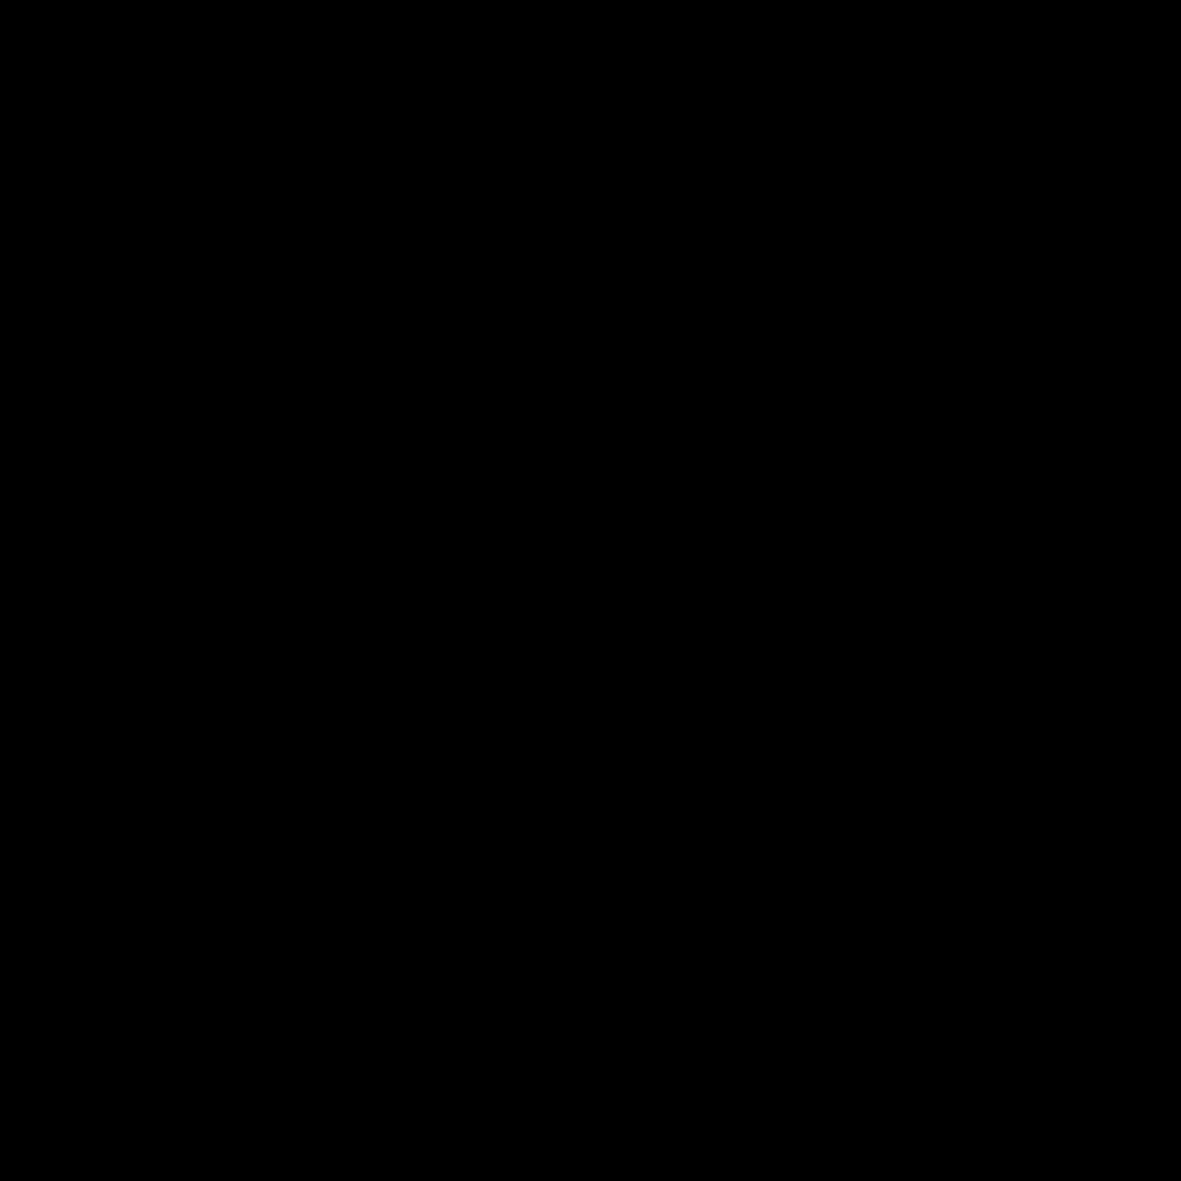
\includegraphics[width=\linewidth]{placeholder-image.png}
%  \caption{Figure 3 caption goes here. Reproduced with permission.\textsuperscript{[Ref.]} Copyright Year, Publisher.}
%  \label{fig:boat1}
%\end{figure}
%
%\begin{table}
% \caption{Table 1 caption}
%  \begin{tabular}[htbp]{@{}lll@{}}
%    \hline
%    Description 1 & Description 2 & Description 3 \\
%    \hline
%    Row 1, Col 1  & Row 1, Col 2  & Row 1, Col 3  \\
%    Row 2, Col 1  & Row 2, Col 2  & Row 2, Col 3  \\
%    \hline
%  \end{tabular}
%\end{table}
%
%
%% Please provide Biographies and photos for Essays, Feature Articles, Progress Reports, Reviews, and Perspectives for those authors who should be highlighted
%% These should be at most 100 words long
%% For other article types this section can be removed
%% Photographs should be 40mm broad and 50 mm high
%
%\begin{figure}
%  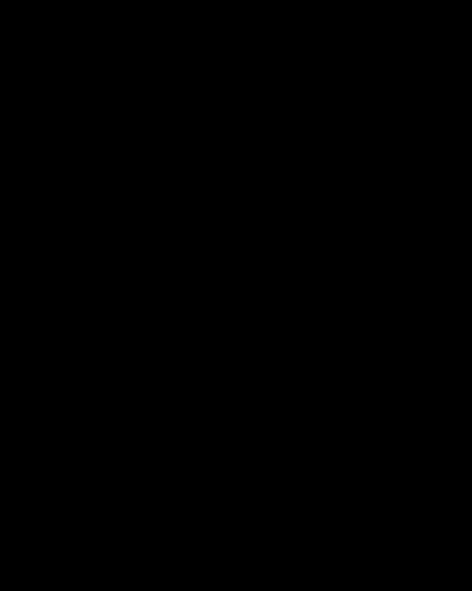
\includegraphics{bio-placeholder.jpg}
%  \caption*{Biography}
%\end{figure}
%
%\begin{figure}
%  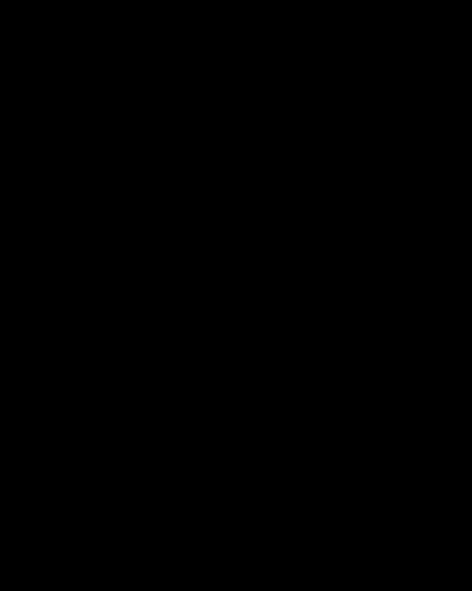
\includegraphics{bio-placeholder.jpg}
%  \caption*{Biography}
%\end{figure}
%
%\begin{figure}
%  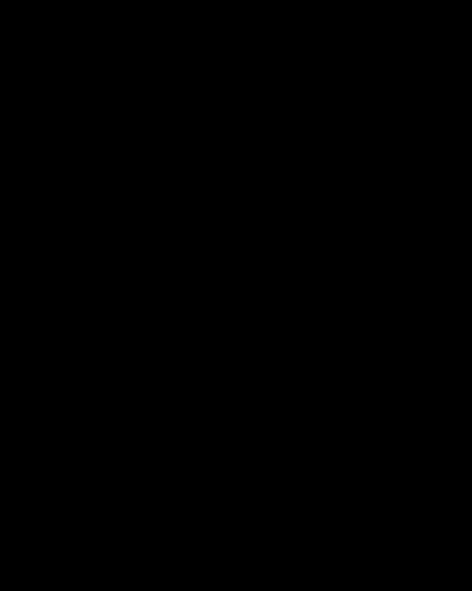
\includegraphics{bio-placeholder.jpg}
%  \caption*{Biography}
%\end{figure}
%
%\begin{figure}
%  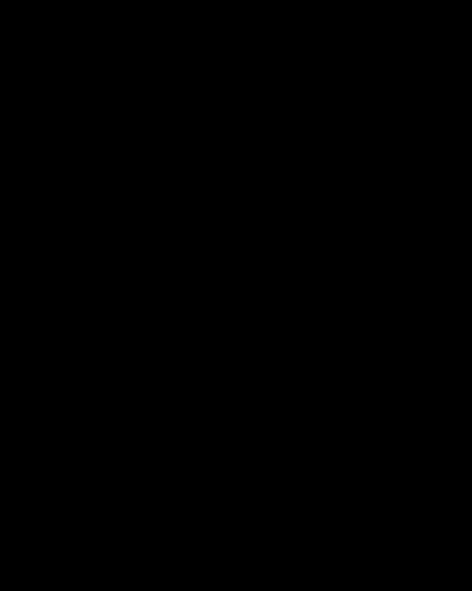
\includegraphics{bio-placeholder.jpg}
%  \caption*{Biography}
%\end{figure}
%
%


%% Table of contents entry should be 50 - 60 words long
%% Image should be 55 mm broad and 50 mm high or 110 mm broad and 20 mm high
%
%
\begin{figure}
\textbf{Table of Contents}\\
\medskip
  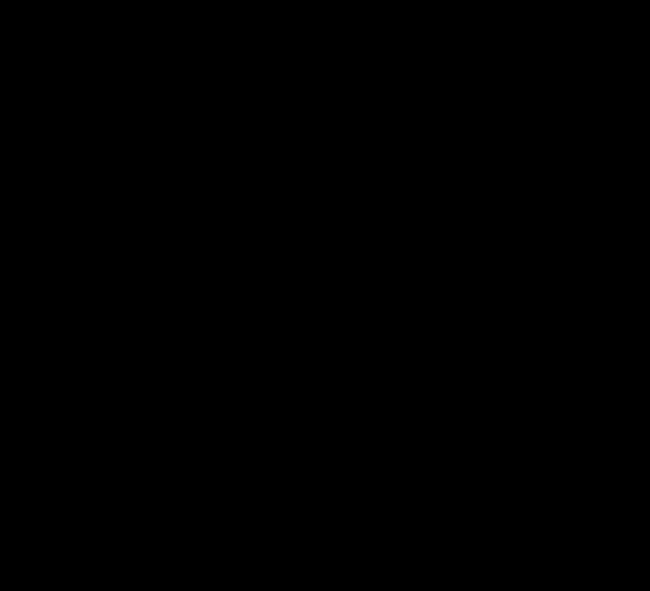
\includegraphics{toc-image.png}
  \medskip
  \caption*{The results of an study on the kinetic of dissociation of FeB pairs in Cz-Si:B using different light sources are reported.
Dissociation rate was shown to depend not only on intensity but also on spectral composition of illumination.
The investigation has revealed increase in the dissociation efficiency with a decrease in wavelength and dominant role of the recombination-enhanced defect reaction}
\end{figure}



\end{document}
